\documentclass[a4paper, 50pt, twoside]{article}
\usepackage[italian]{babel}
\usepackage[a4paper, top=2cm, bottom=2cm, left=3cm, right=3cm]{geometry}
\usepackage{graphicx}
\graphicspath{{immagini/}}
\usepackage{chngcntr}
\counterwithin{figure}{section}
\usepackage{braket}
\usepackage{amsmath}
\usepackage{fancyhdr}
\usepackage{xcolor}
\usepackage{listings}
\usepackage{pxfonts}
\pagestyle{fancy}
\lfoot{EasyVersity}

\definecolor{grigio}{rgb}{0.85,0.85,0.85}
\lstset{
language = Java,
basicstyle = \ttfamily \small,
keywordstyle = \bfseries,
numbers = left,
backgroundcolor = \color{grigio},
showstringspaces = false,
tabsize = 2
}

\begin{document}


\title{EasyVersity}
\date{Settembre, 2019}
\author{Tomassini Danilo \\ Cappella Simone \\ Mannini Luca \\ \\ Ingegneria Informatica e dell'Automazione}
\maketitle
\vspace*{\fill}
\begin{figure}[h!]
	\centering
	
\includegraphics[width=\linewidth]{copertina4.jpg}
	\label {fig::copertina}
\end{figure}
\vspace*{\fill}

\newpage
\tableofcontents{}

\newpage
\section{Obbiettivi}
EasyVersity rappresenta uno strumento di supporto per lo studente.

Permette di gestire:
\begin{itemize}
\item \textbf{Orario:} salva l'orario delle lezioni nella tua applicazione per consultarlo quando vuoi.
\item \textbf{Archivio appunti locale:} da la possibilità di salvare appunti raggruppandoli per materia, indicando titolo e data si può contestualizzare al meglio l'appunto in questione.
\item \textbf{Condivisione appunti:} rende possibile la condivisione ed il download degli appunti.
\item \textbf{Impostazioni:} da qui si possono cambiare informazioni come username e password, eprendere visione di info "about us".
\end{itemize}

\section{Funzionalità}
Avviata l'applicazione ci si trova davani alla \textbf{First activity}; qui si può scegliere di effettuare il login o registrarsi. Una volta effettuato il login si può accedere al menù principale che prevede 4 scelte:
\begin{itemize}
\item \textbf{Orario.}
\item \textbf{I miei appunti.}
\item \textbf{Appunti condivisi.}
\item \textbf{Impostazioni.}
\end{itemize}
\begin{figure}[!h]
	\centering
	{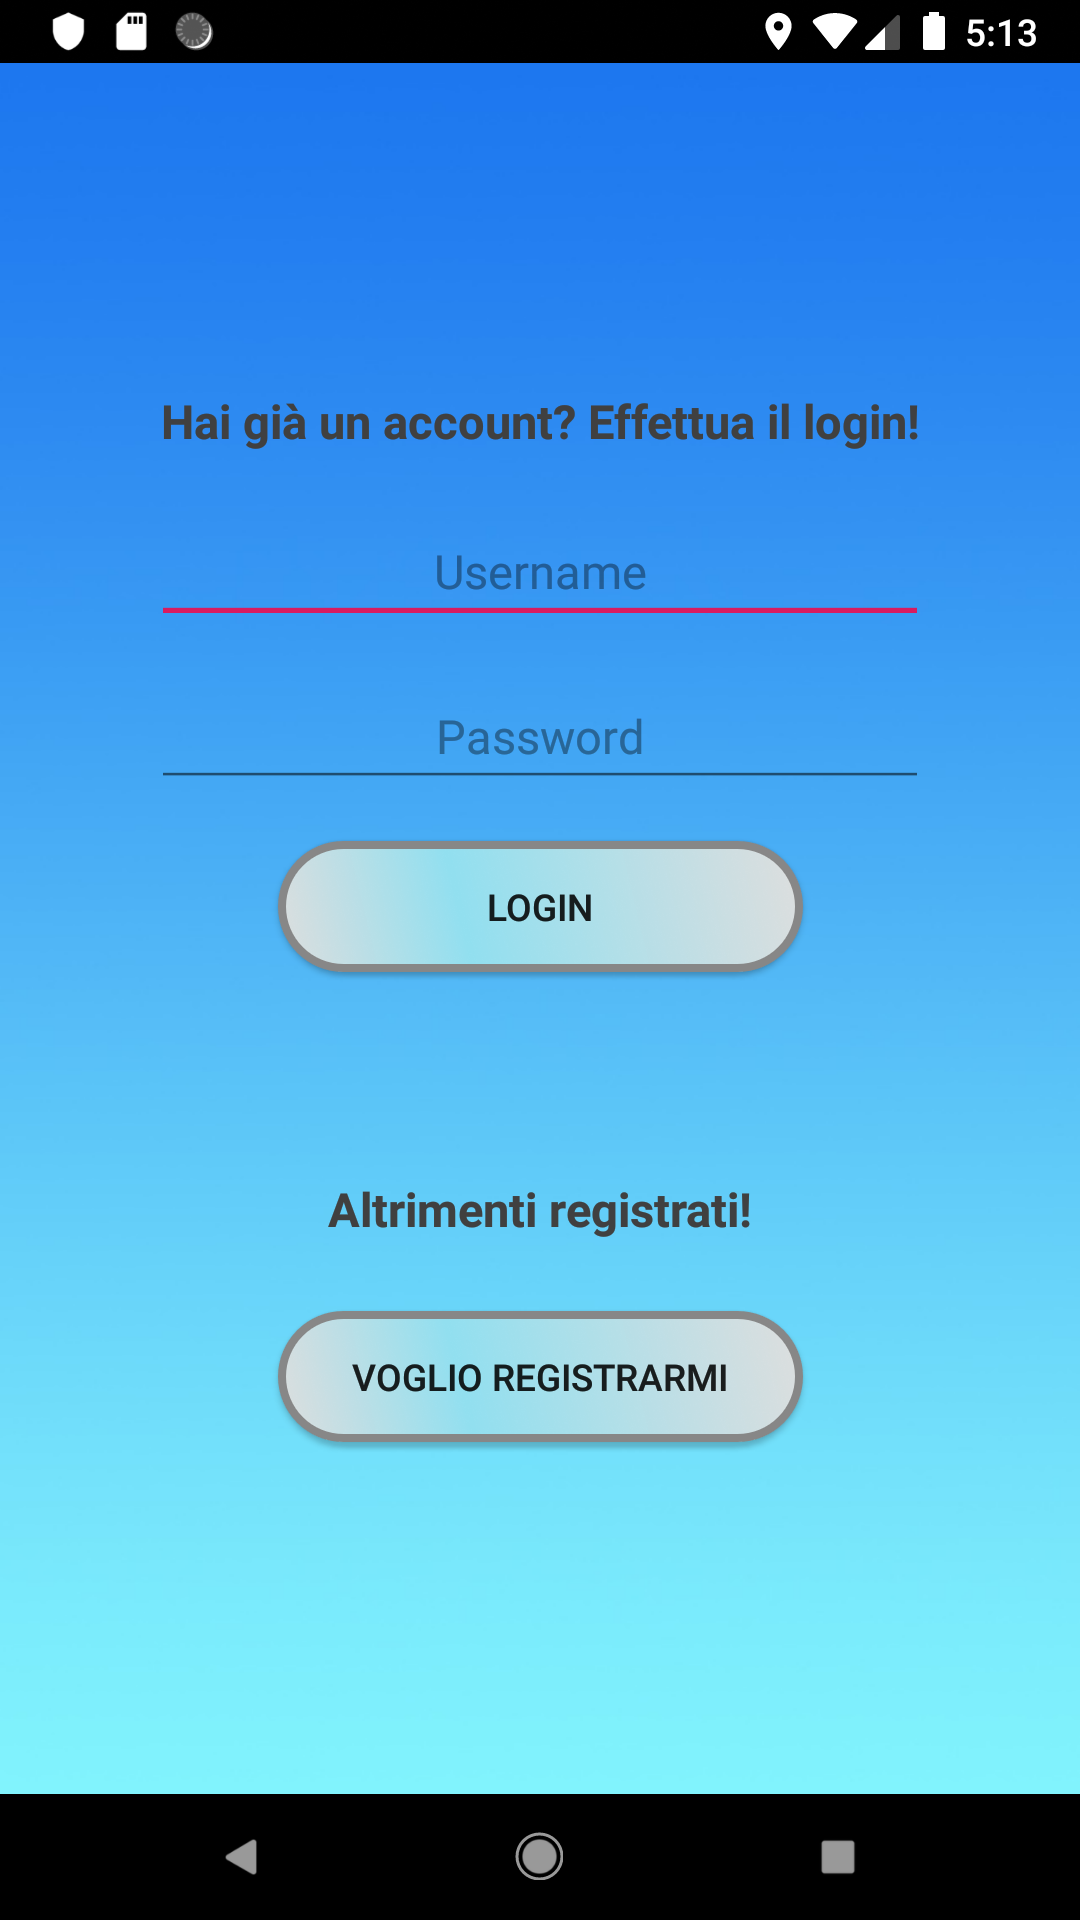
\includegraphics[width=.30\textwidth]{login}} \quad
	{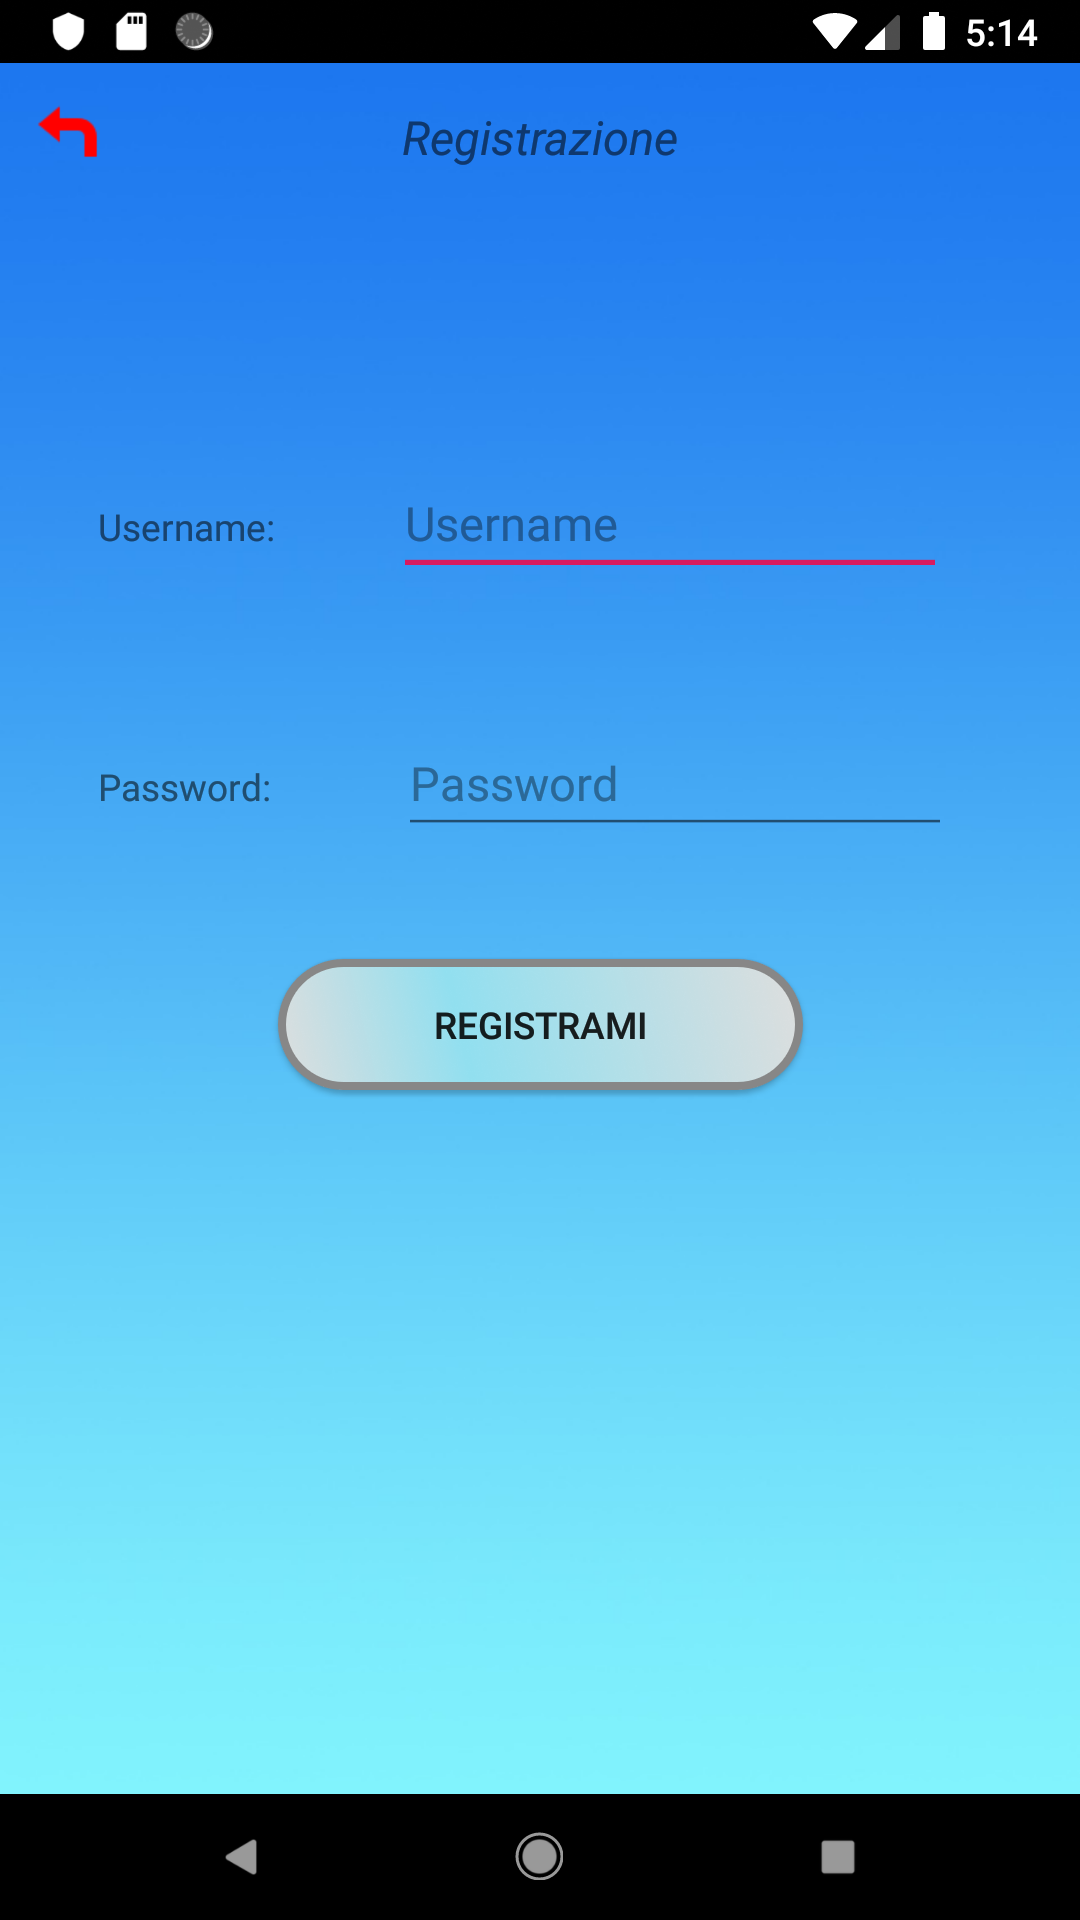
\includegraphics[width=.30\textwidth]{registrazione}} \quad
	{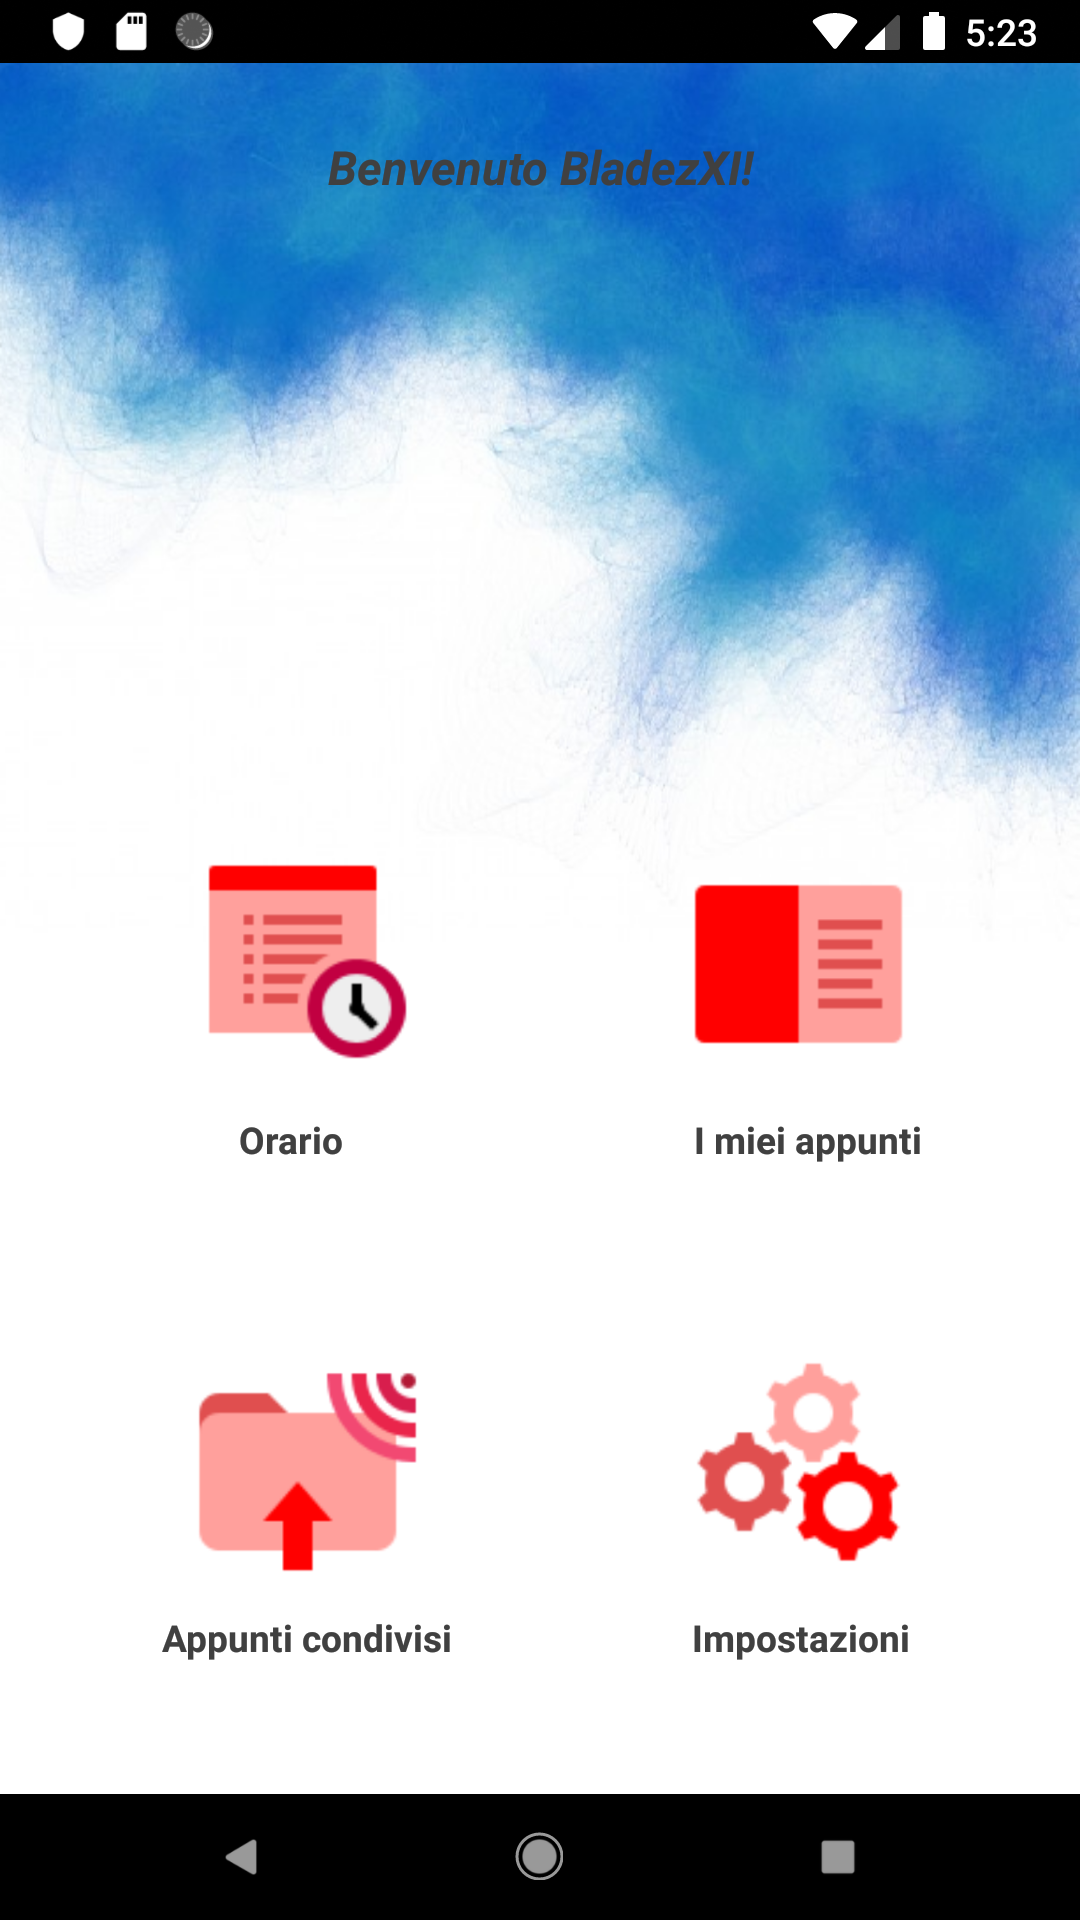
\includegraphics[width=.30\textwidth]{menu}}
	\caption{\small Schermata Login, Registrazione e Menu principale.}
\end{figure}

\newpage
\subsection{Orario}
Aperto l'orario ci si trova di fronte alla tabella relativa al giorno corrente; con la bottom navbar si può scegliere il giorno su cui andare ad agire.
Premendo nel campo \textbf{materia}, relativo all'ora di interesse si può inserire la materia in tabella, si accede, infatti, ad una lista predefinita di materie (questa può essere estesa scegliendo di inserirne una manualmente con il bottone "altro"). Scelta la materia viene visualizzata una finestra di dialogo che permette di inserire l'aula in cui si svolgerà la lezione e la durata della stessa.
\begin{figure}[!h]
	\centering
	{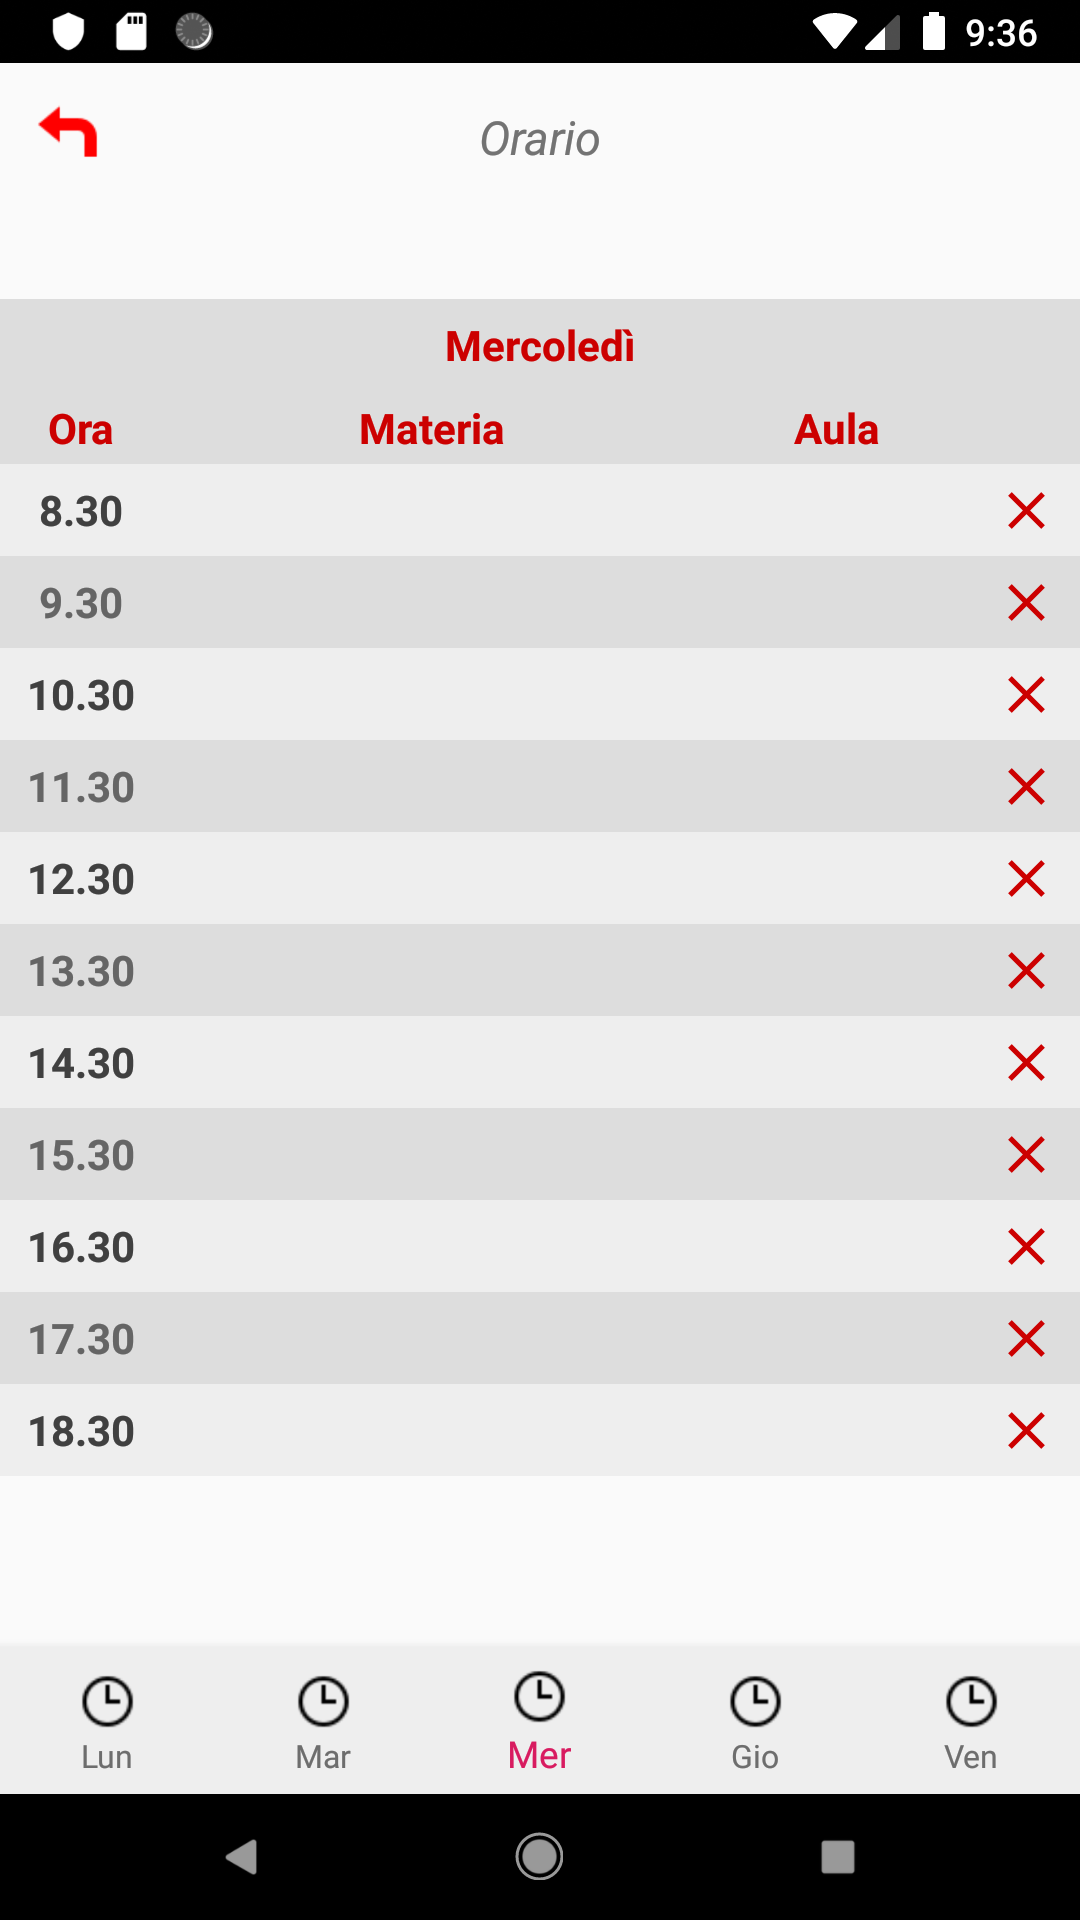
\includegraphics[width=.30\textwidth]{orario}} \quad
	{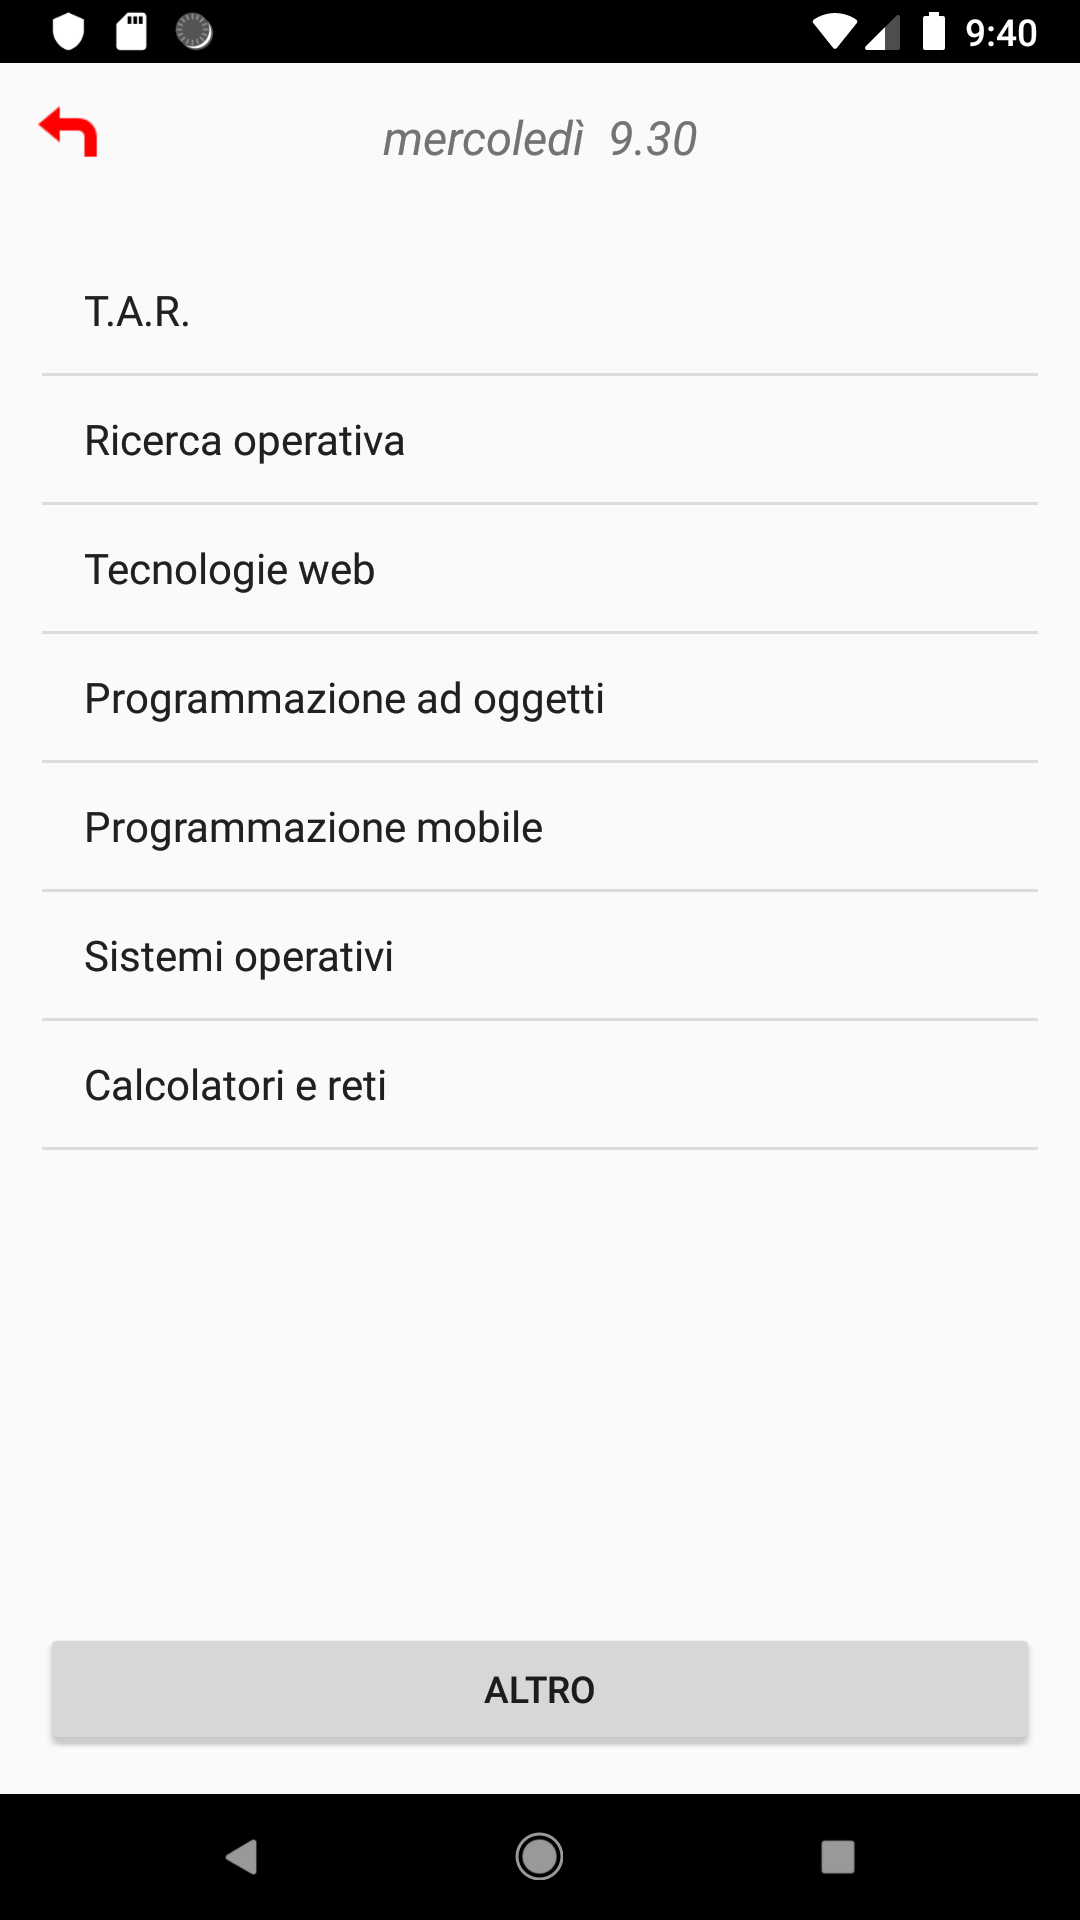
\includegraphics[width=.30\textwidth]{orario_scelta_materia}}\quad
	{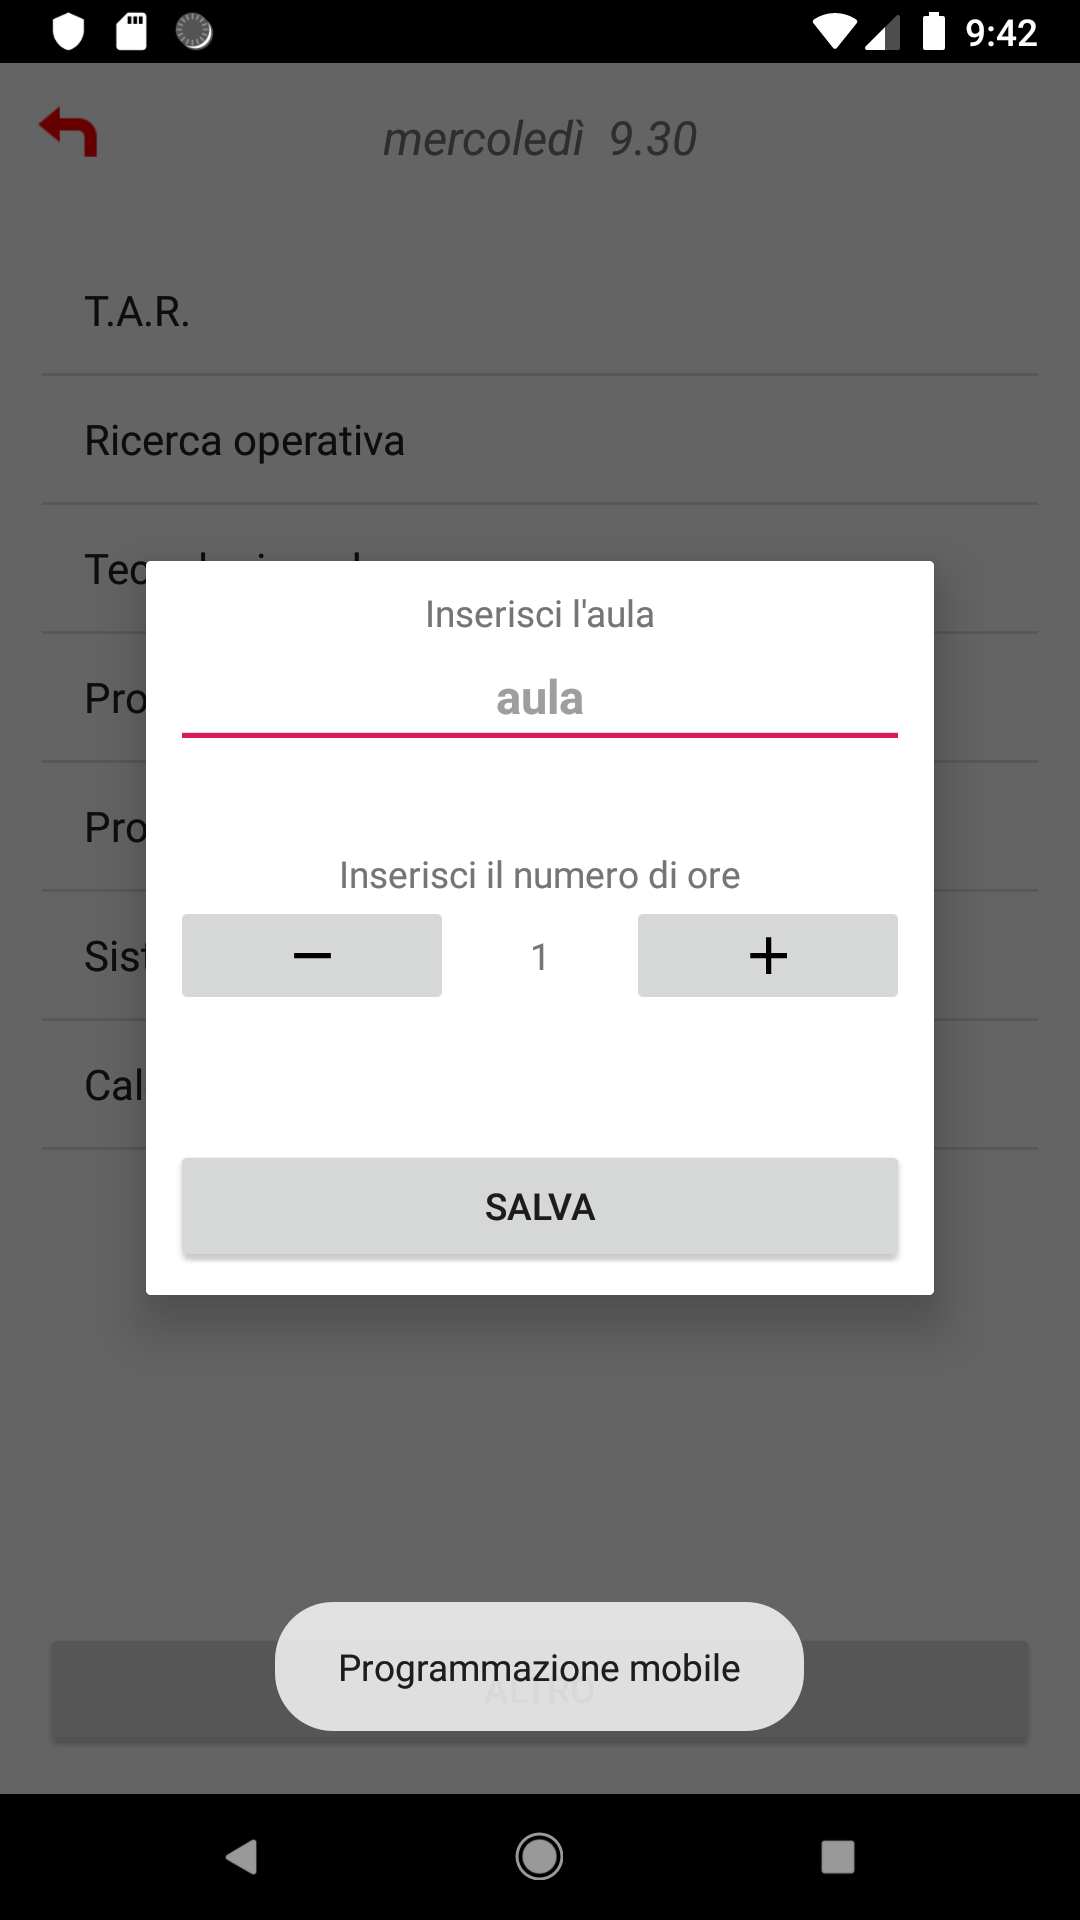
\includegraphics[width=.30\textwidth]{orario_inserimento}}
	\caption{\small Orario.}
\end{figure}

Salvata la materia nell'orario questa viene salvata nel database e inserita in una lista nella sezione \textbf{i miei appunti}.

\subsection{I miei appunti}
In questa sezione abbiamo accesso alla lista di tutte le materie salvate nel database. Abbiamo la possibilità di aggiungerne altre a piacimento o eliminarle inserendo il nome esatto della materia.

\begin{figure}[!h]
	\centering
	{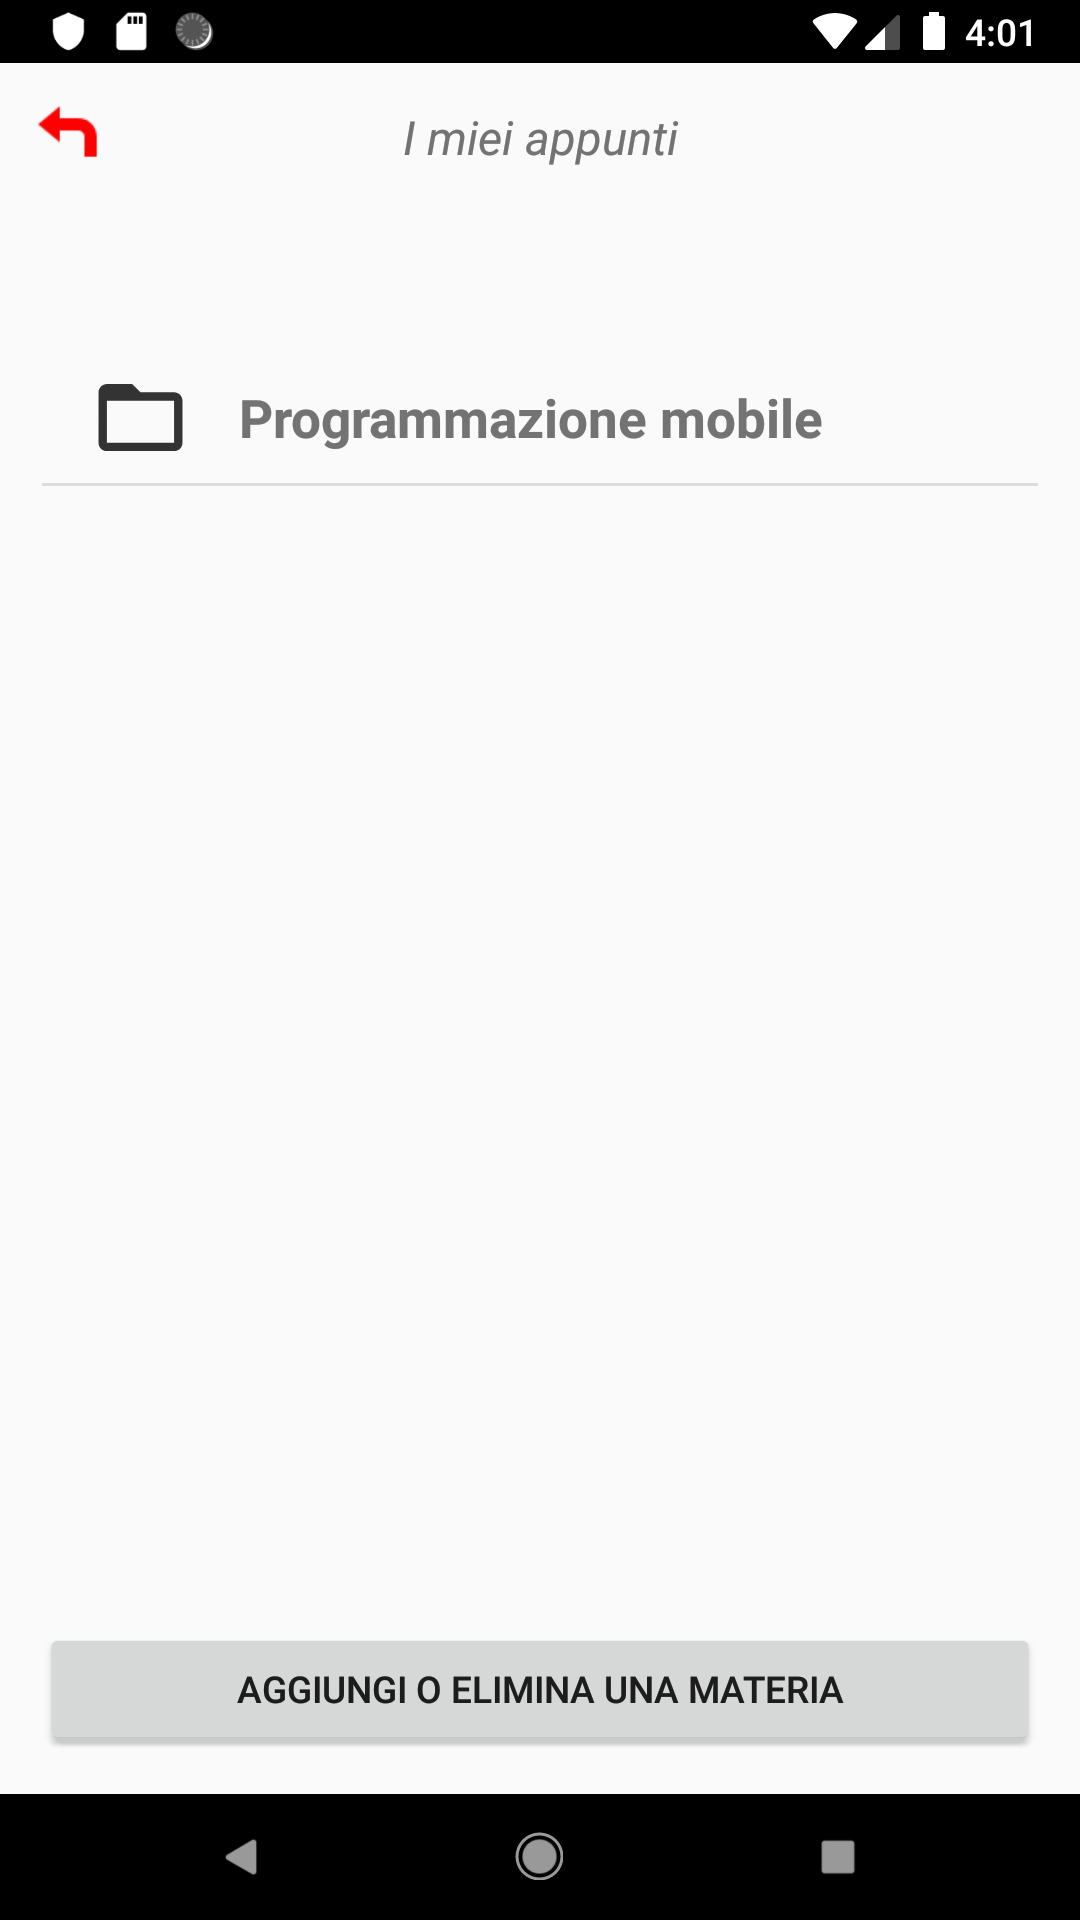
\includegraphics[width=.30\textwidth]{miei_appunti_lista_materie}} \quad
	{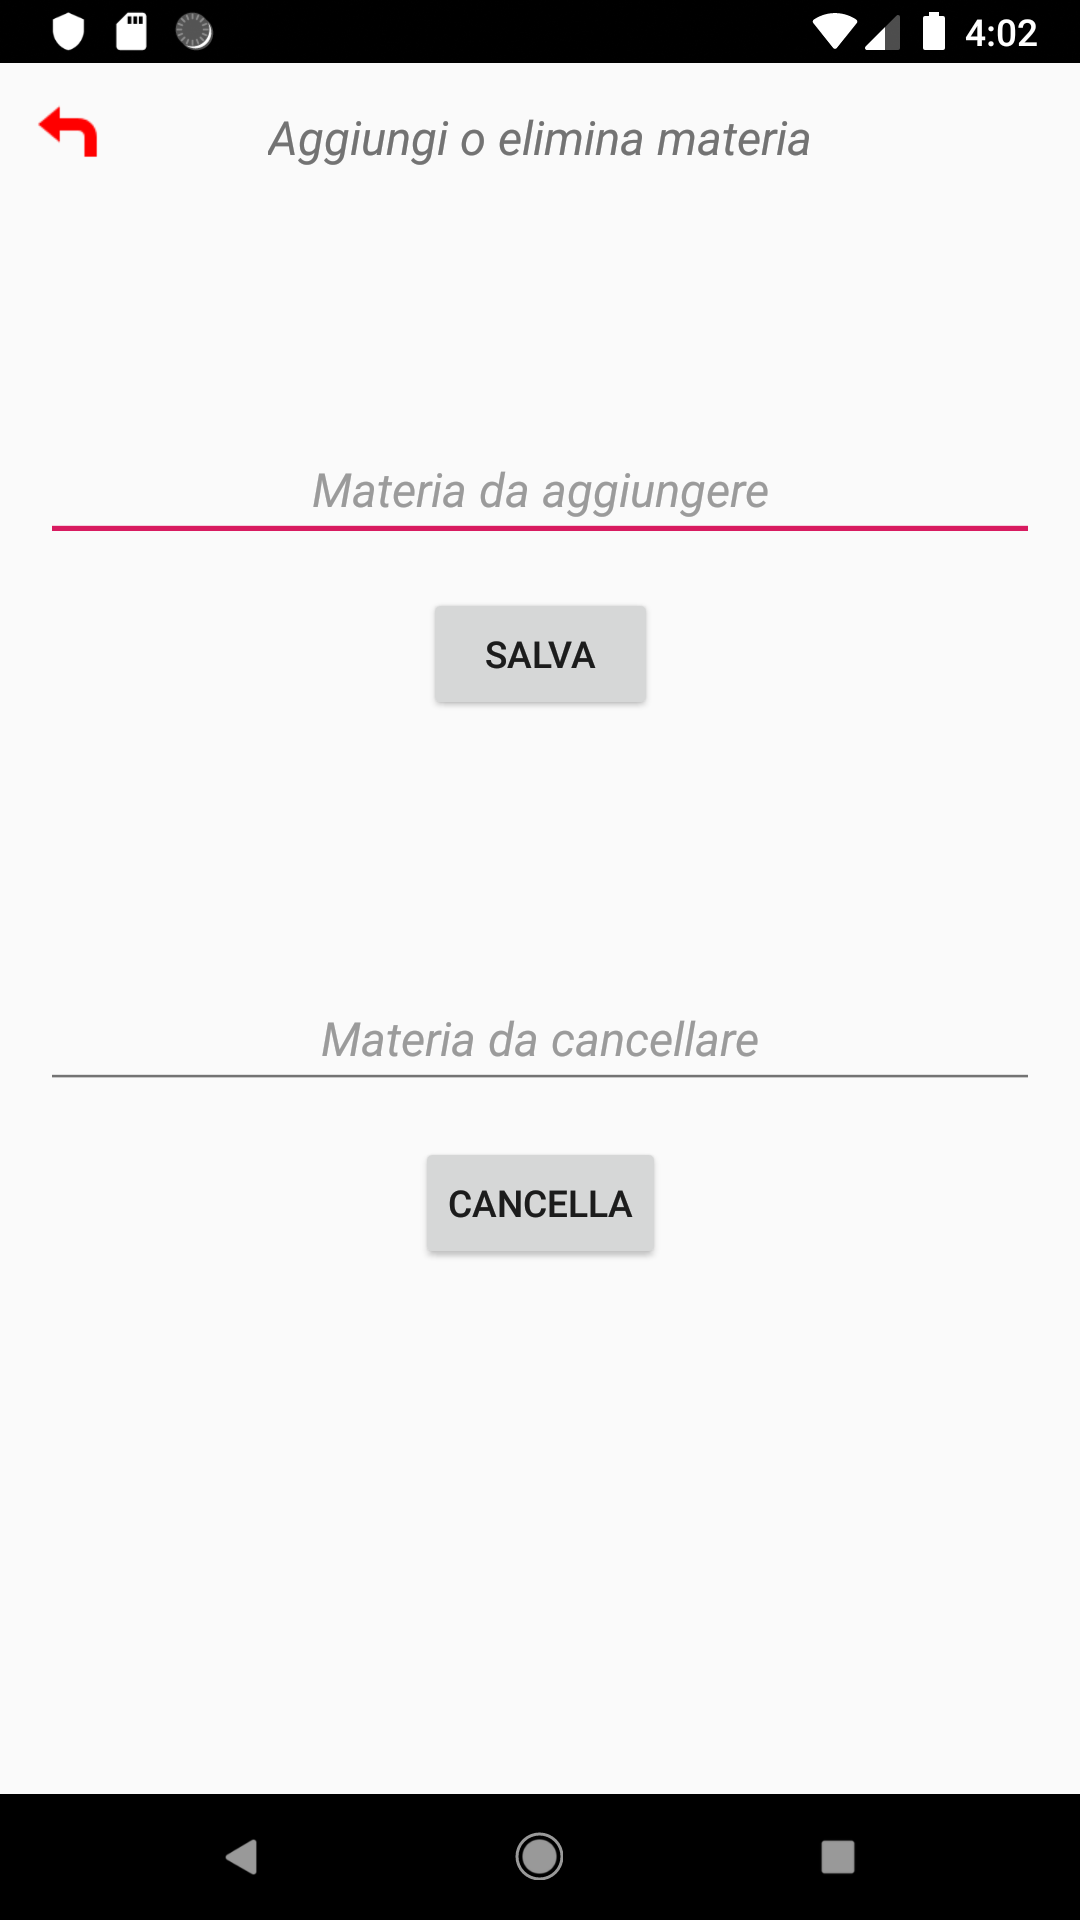
\includegraphics[width=.30\textwidth]{miei_appunti_aggiungi_materia}} \quad
	{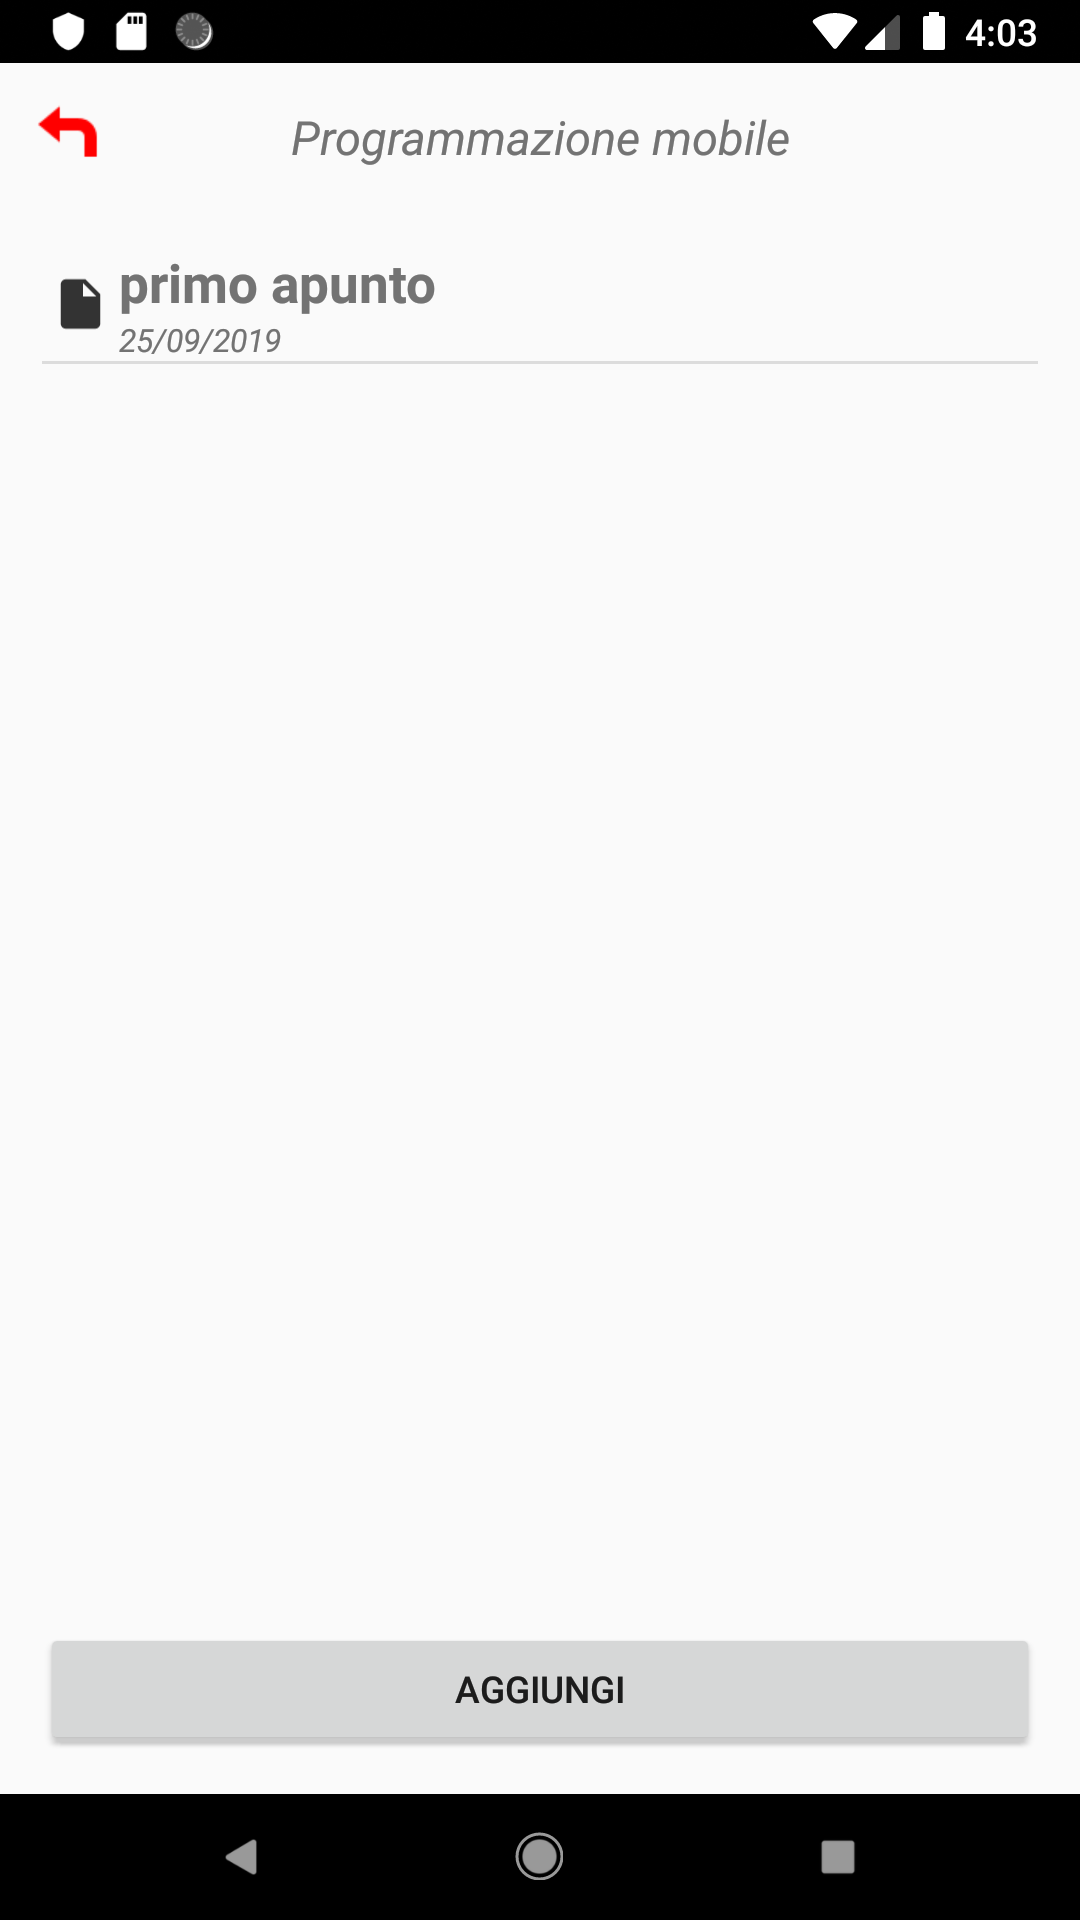
\includegraphics[width=.30\textwidth]{miei_appunti_lista_appunti}}
	\caption{\small Scegli aggiungi o elimina una materia e scegli un appunto.}
\end{figure}

Scelta la materia accediamo ad una seconda lista contenente tutti gli appunti relativi ad essa; ogni elemento della lsita contiene titolo e data relativi ad ogni appunto.
Da questa lista possiamo accedere e visualizzare l'annotazione vera e propria.

Gli appunti possono essere aggiunti con il bottone \textbf{"aggiungi"}, qui inseriremo titolo data e annotazione che vogliamo salvare; da questa schermata, inserendo la spunta nel campo \textbf{"Condividi"}, possono essere condivisi direttamente gli appunti con gli altri utenti.

Per eliminare un appunto basta tenere premuto l'elemento da eliminare, verrà attivata una finestra di dialogo da cui è possibile confermare la cancellazione.

\begin{figure}[!h]
	\centering
	{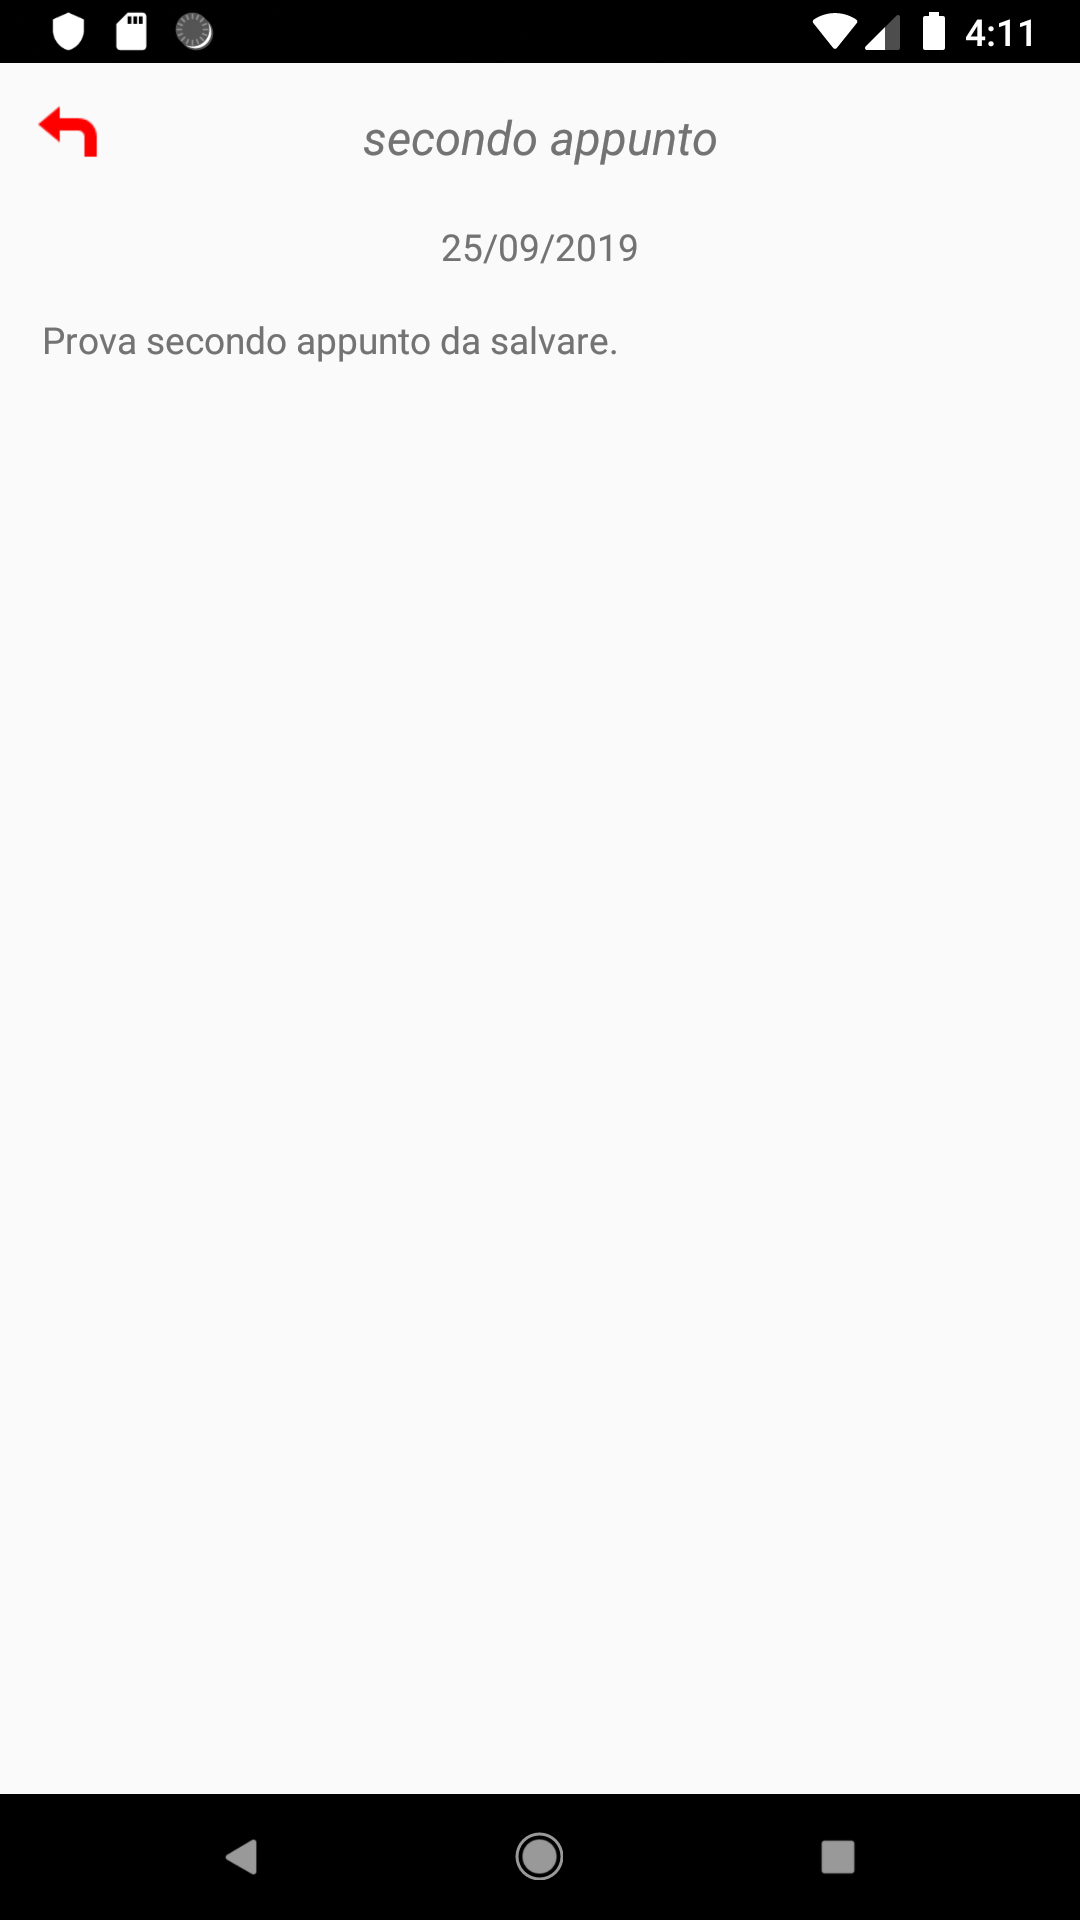
\includegraphics[width=.30\textwidth]{miei_appunti_vedi_appunto}} \quad
	{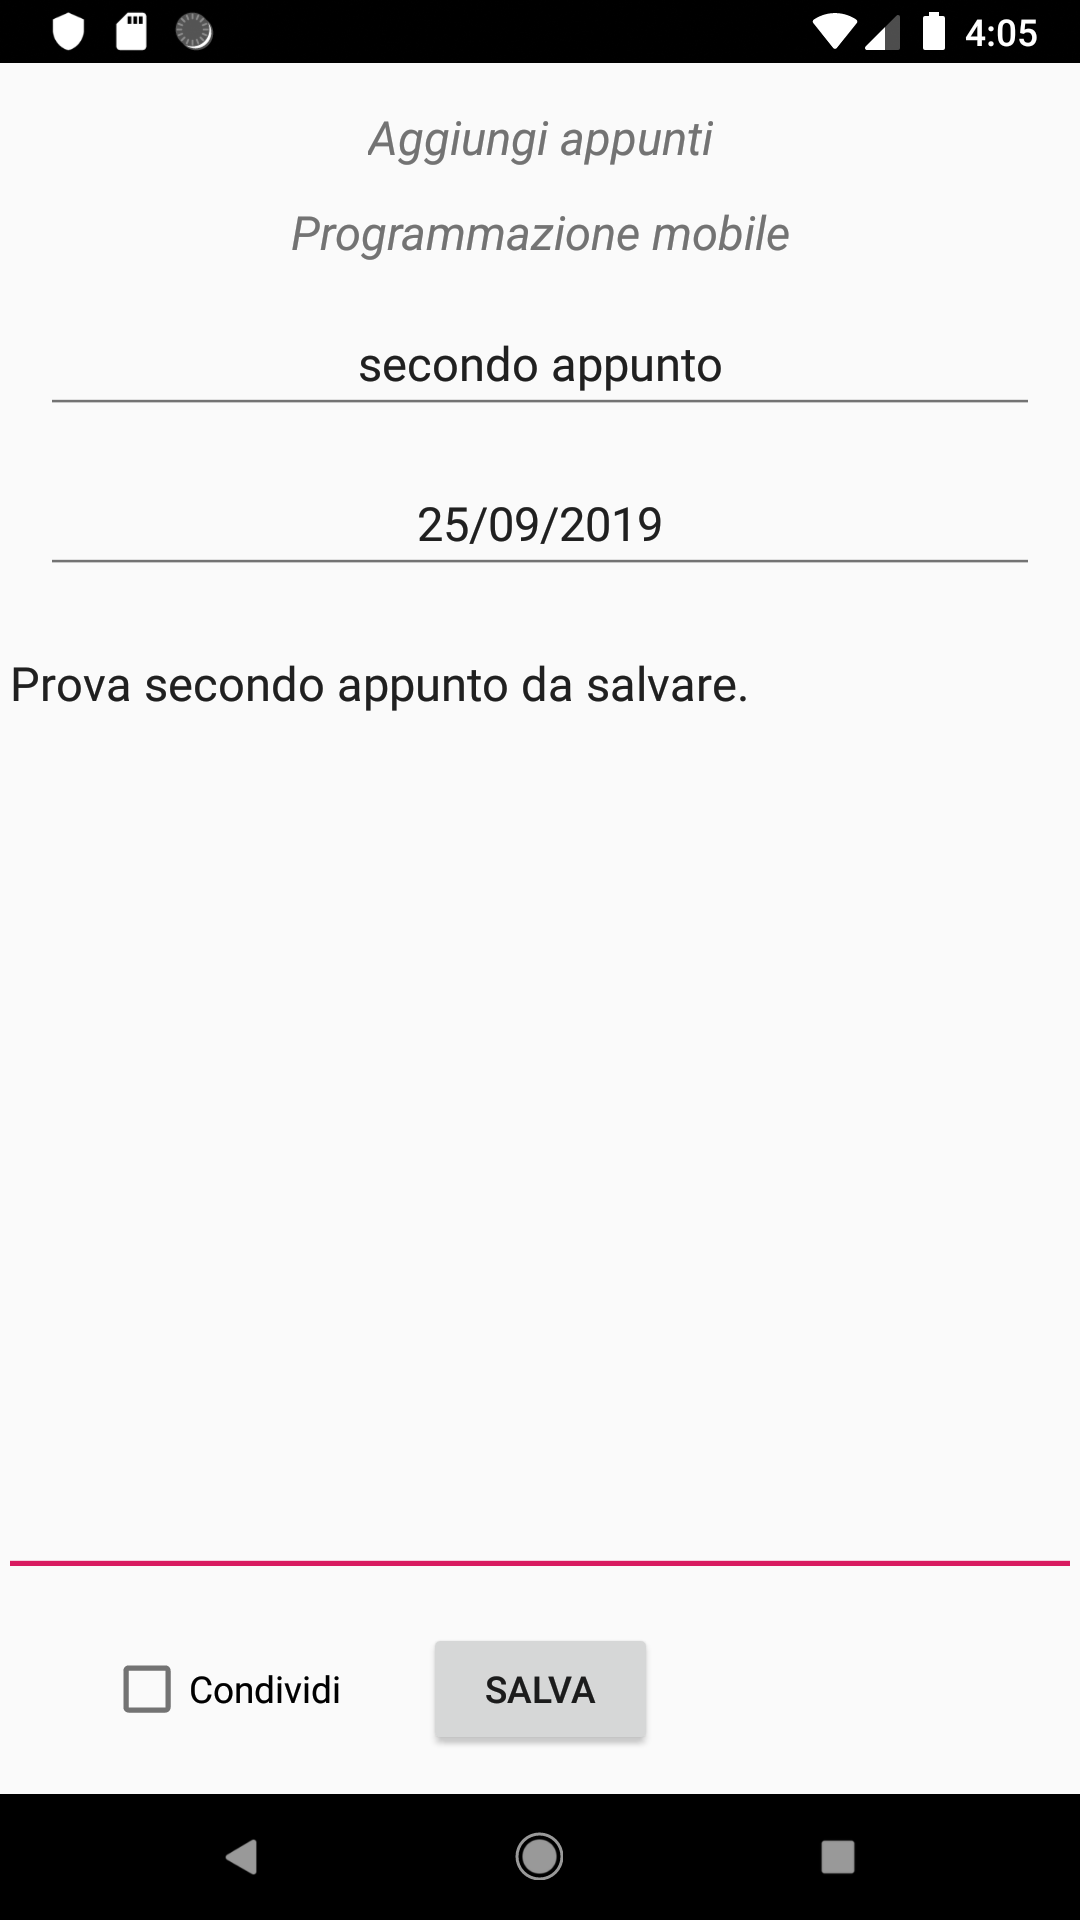
\includegraphics[width=.30\textwidth]{miei_appunti_aggiungi_appunto}} \quad
	{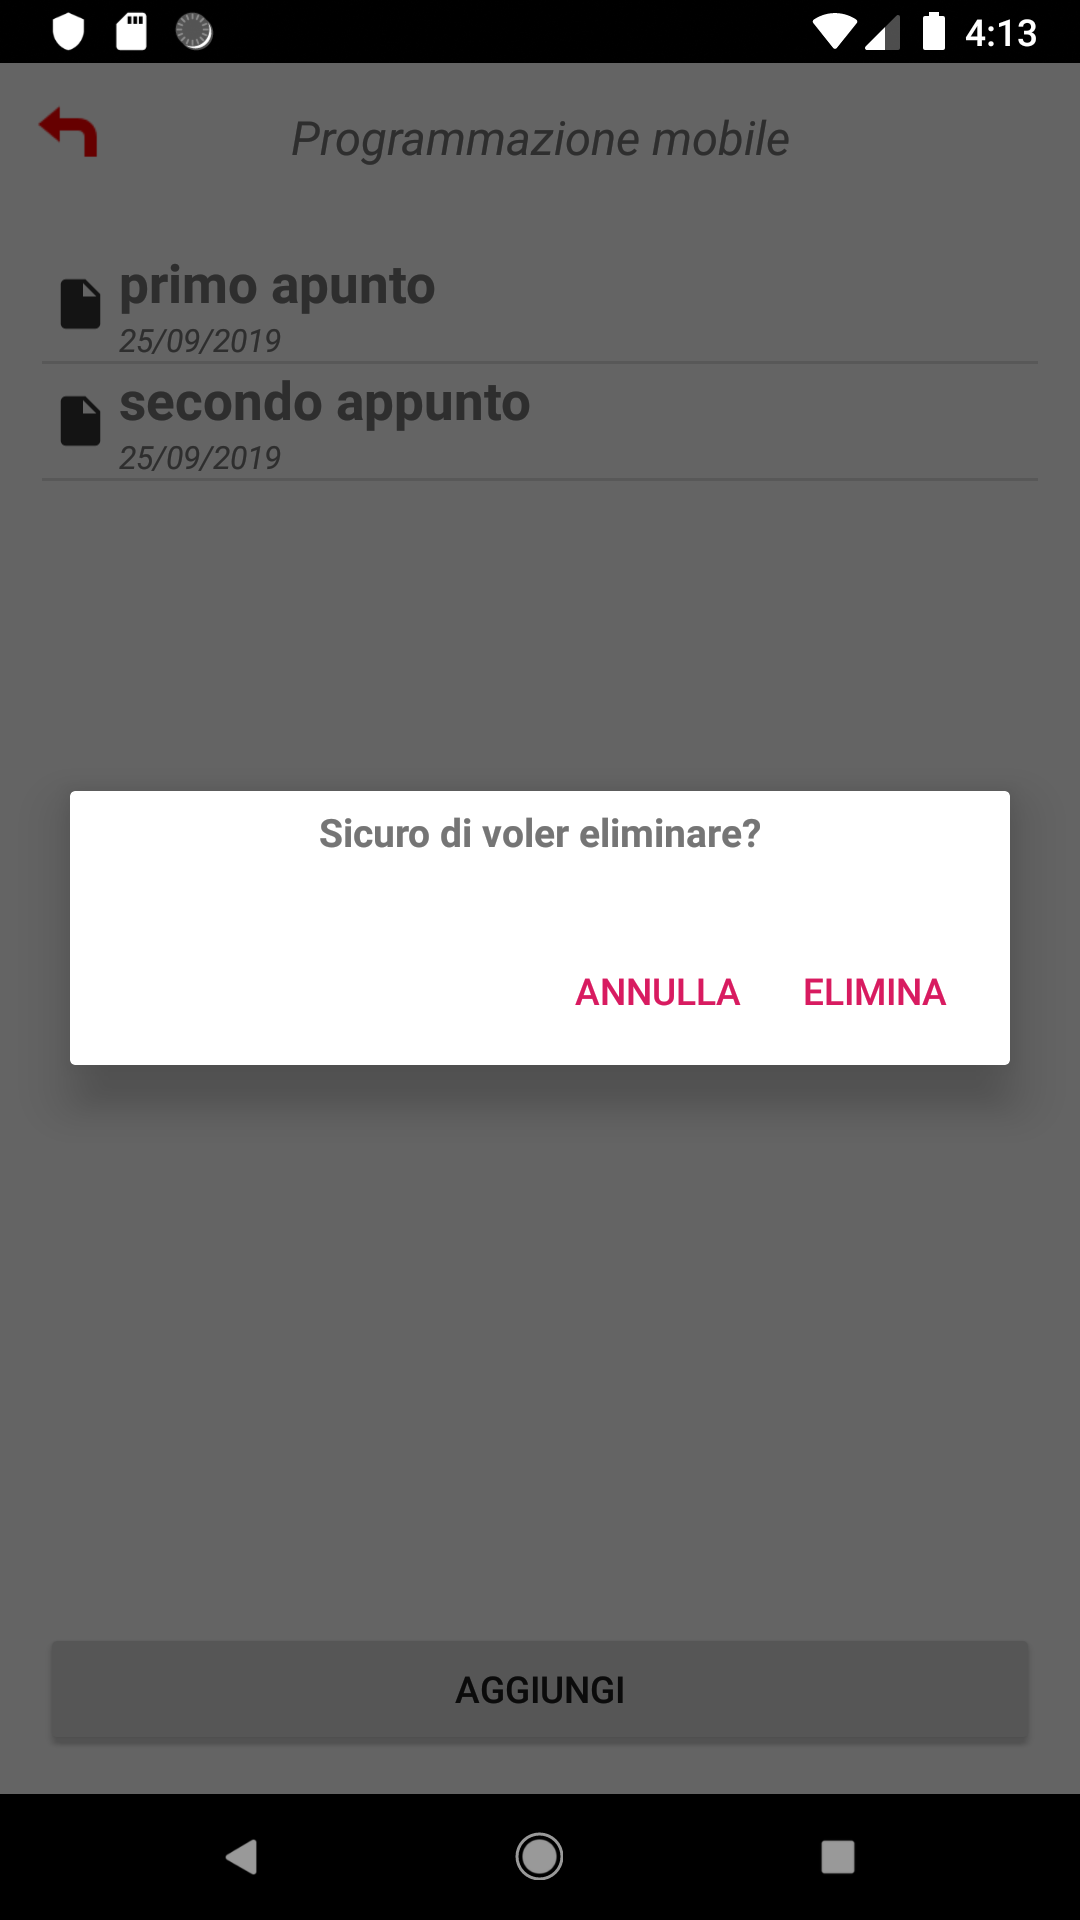
\includegraphics[width=.30\textwidth]{miei_appunti_elimina_appunto}}
	\caption{\small Visualizza, aggiungi o elimina un appunto.}
\end{figure}

\subsection{Appunti condivisi}
Nella sezione appunti condivisi possiamo scegliere una delle materie predefinite in lista per visualizzare gli appunti che sono stati condivisi ed eventualmente visualizzarli o scaricarli.

\begin{figure}[!h]
	\centering
	{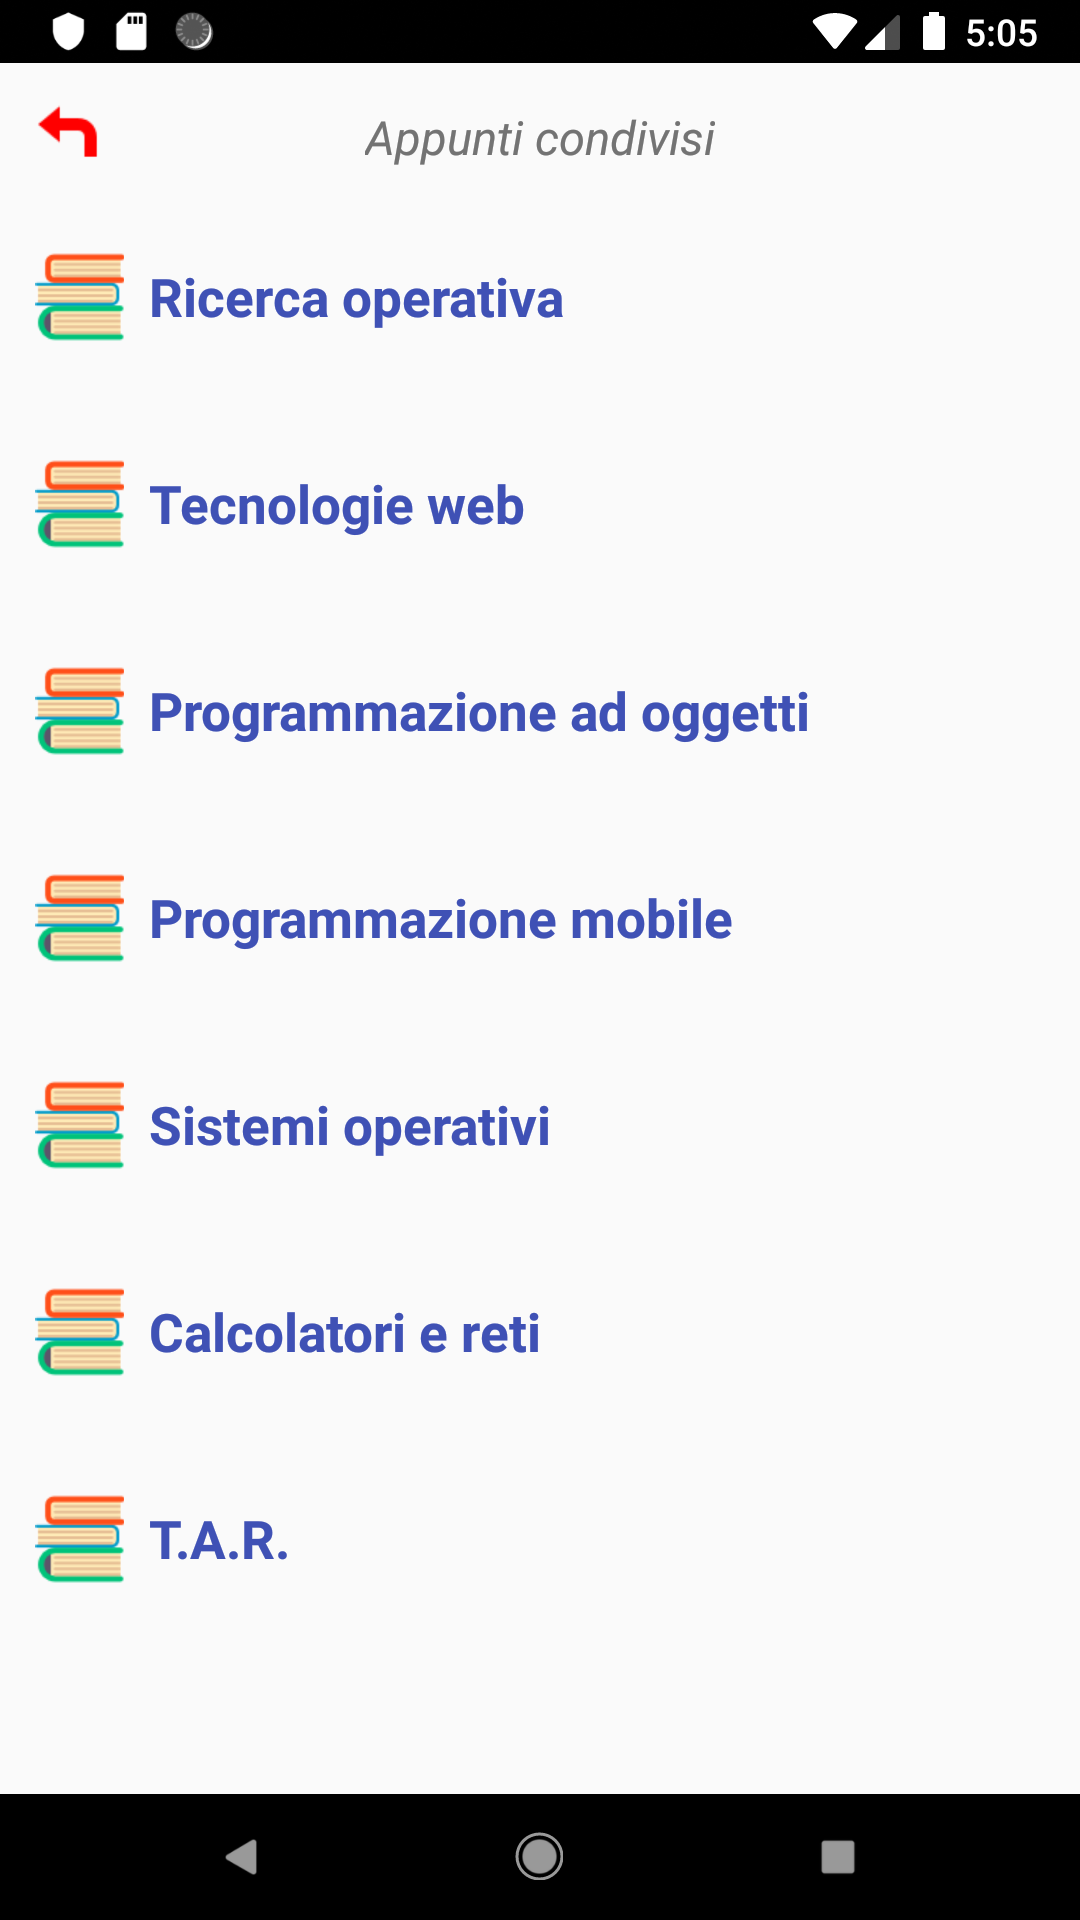
\includegraphics[width=.30\textwidth]{appunti_condivisi_lista_materie}} \quad
	{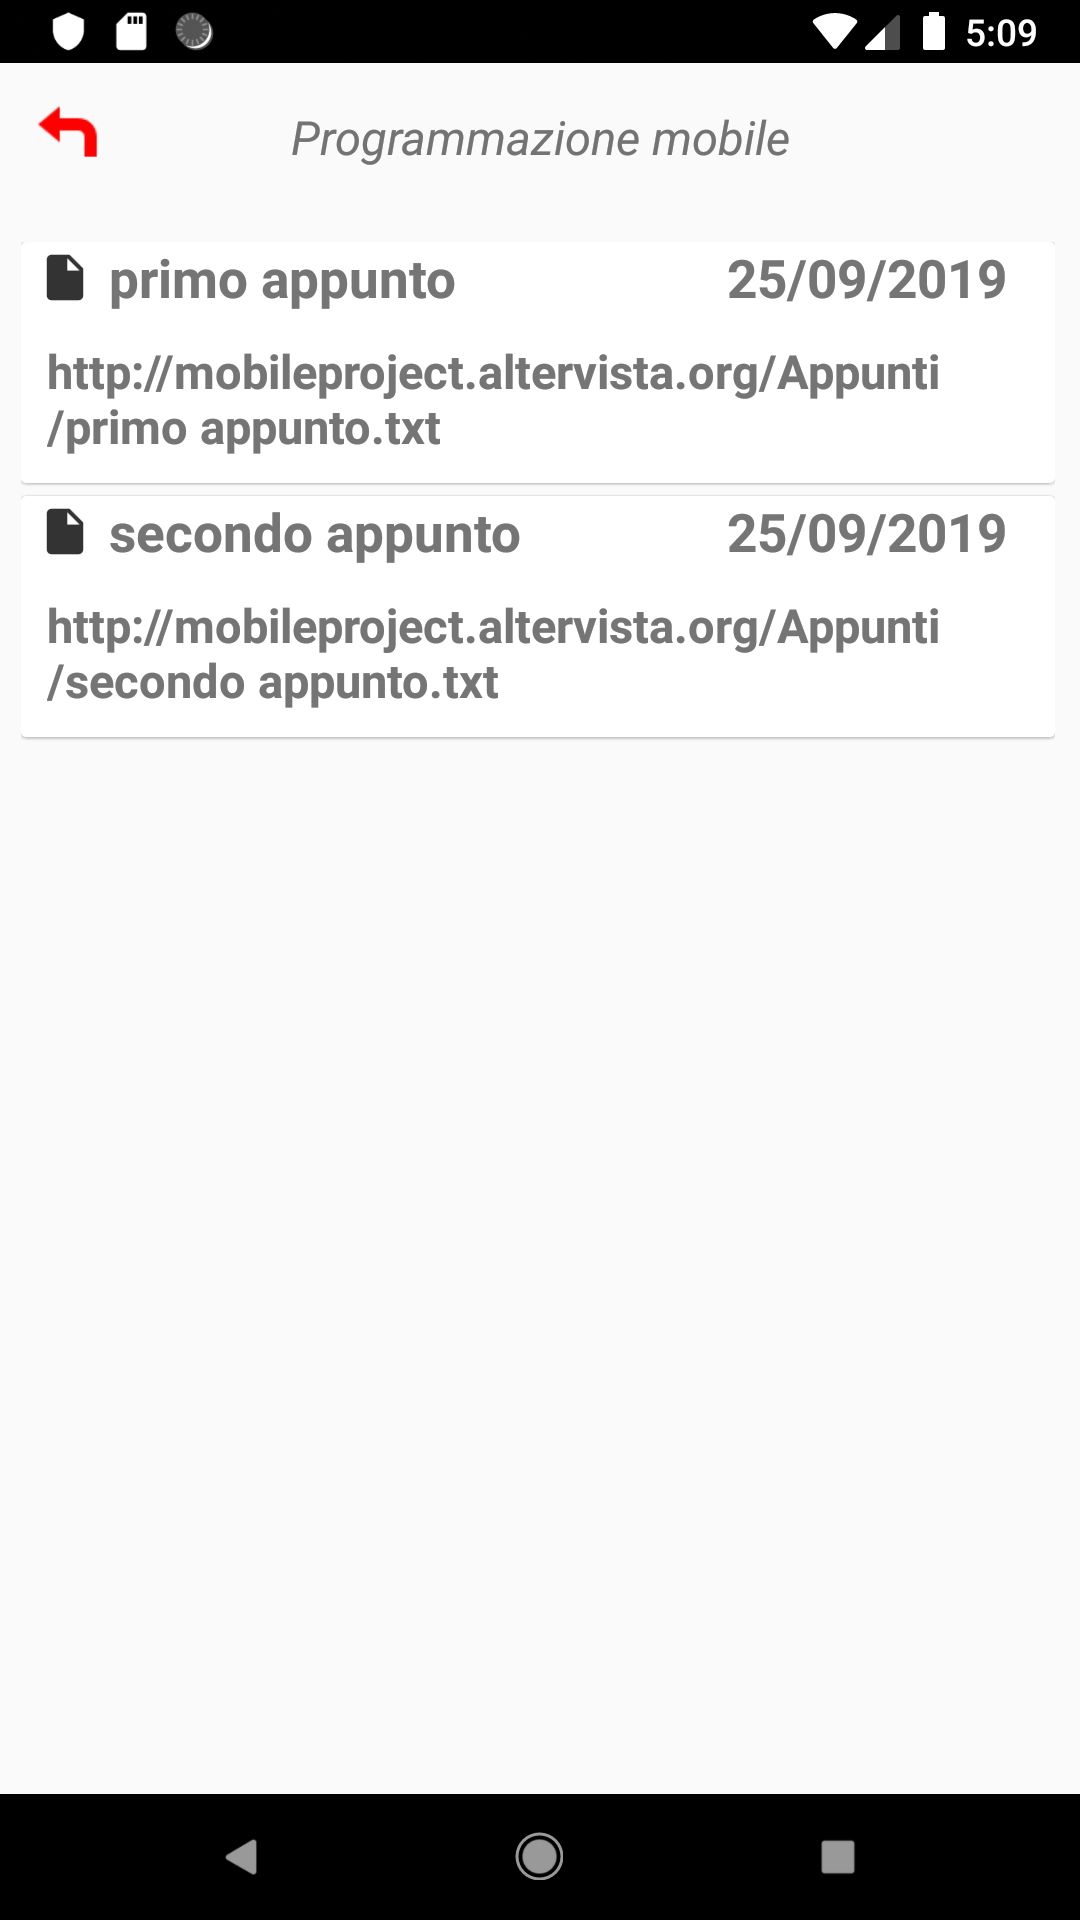
\includegraphics[width=.30\textwidth]{appunti_condivisi_lista_appunti}} \quad
	{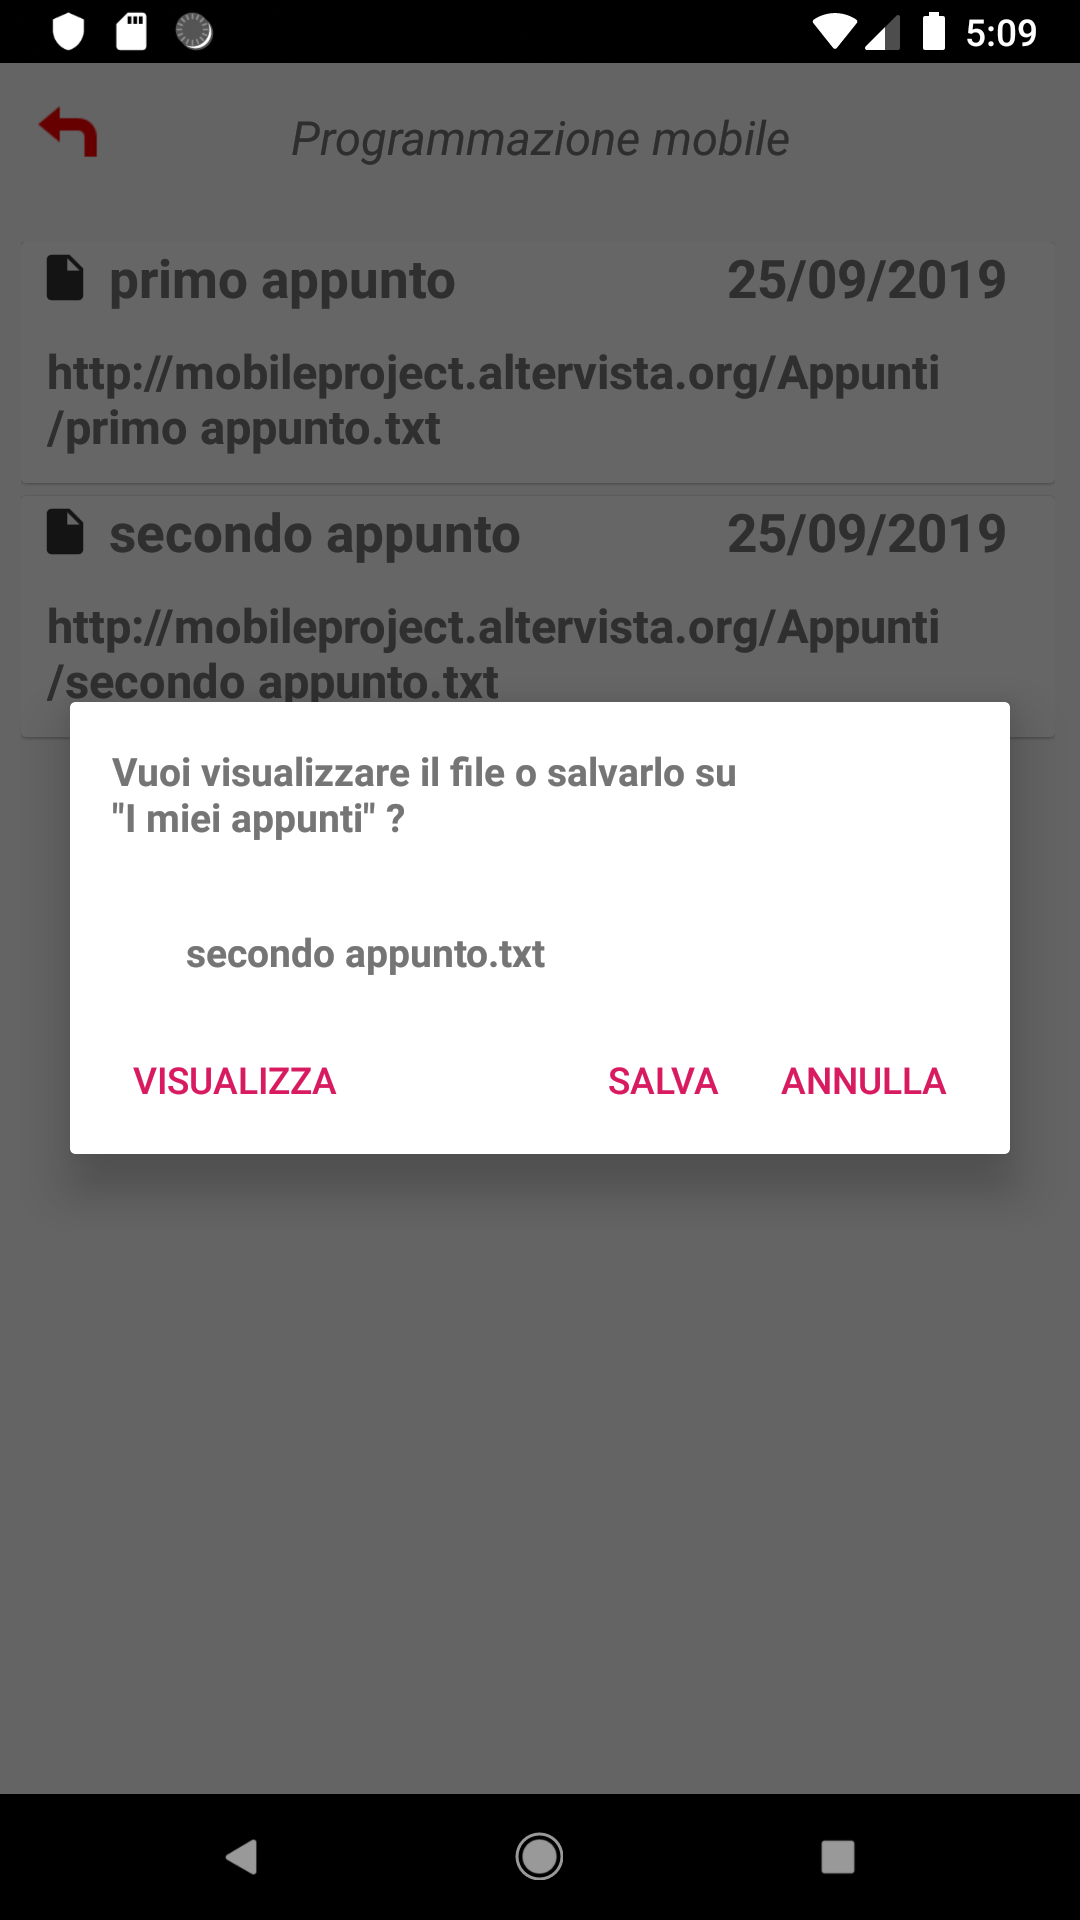
\includegraphics[width=.30\textwidth]{appunti_condivisi_scegli_azione}}
	\caption{\small Appunti condivisi, scegli la materia, scegli l'appunto, visualizza o scarica.}
\end{figure}

\subsection{Impostazioni}
Dalle impostazioni possiamo banalmente modificare \textbf{username}, \textbf{password} e leggere informazioni \textbf{about us}.

\begin{figure}[!h]
	\centering
	{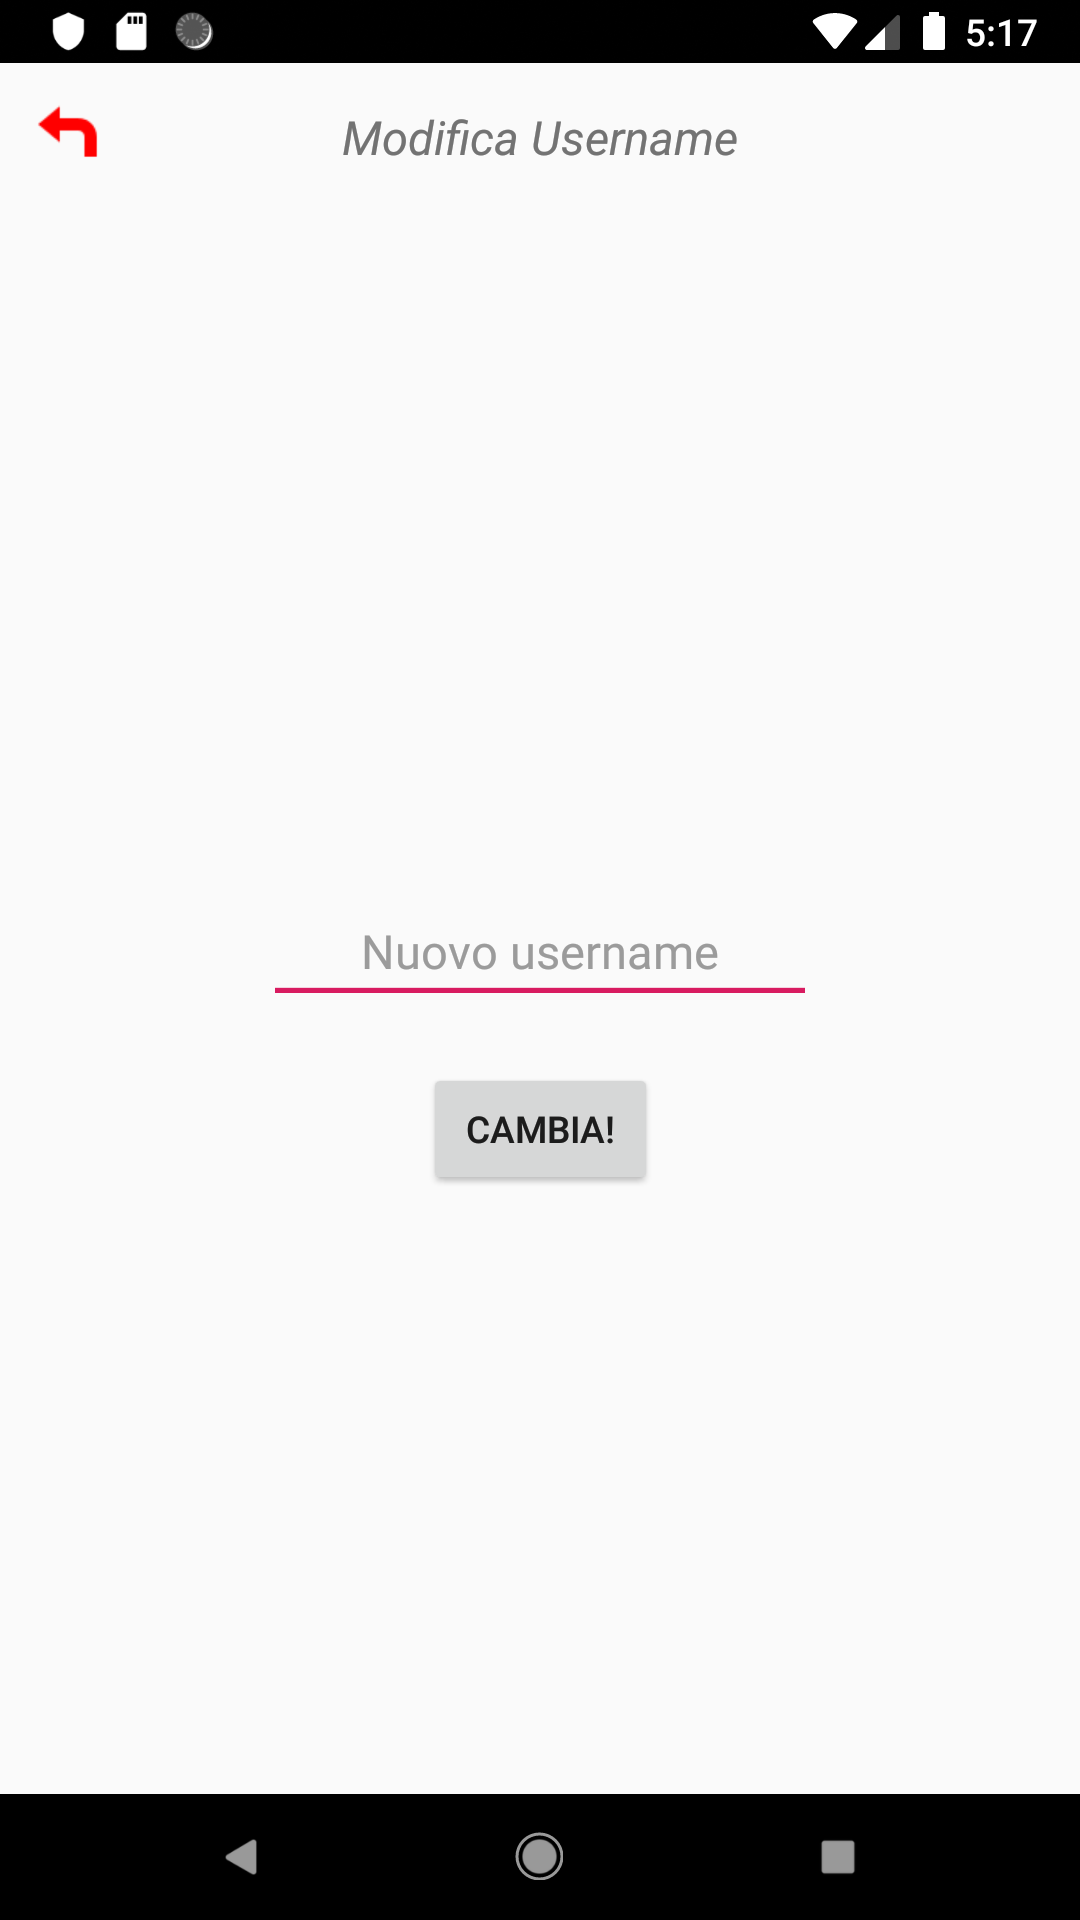
\includegraphics[width=.30\textwidth]{impostazioni_username}} \quad
	{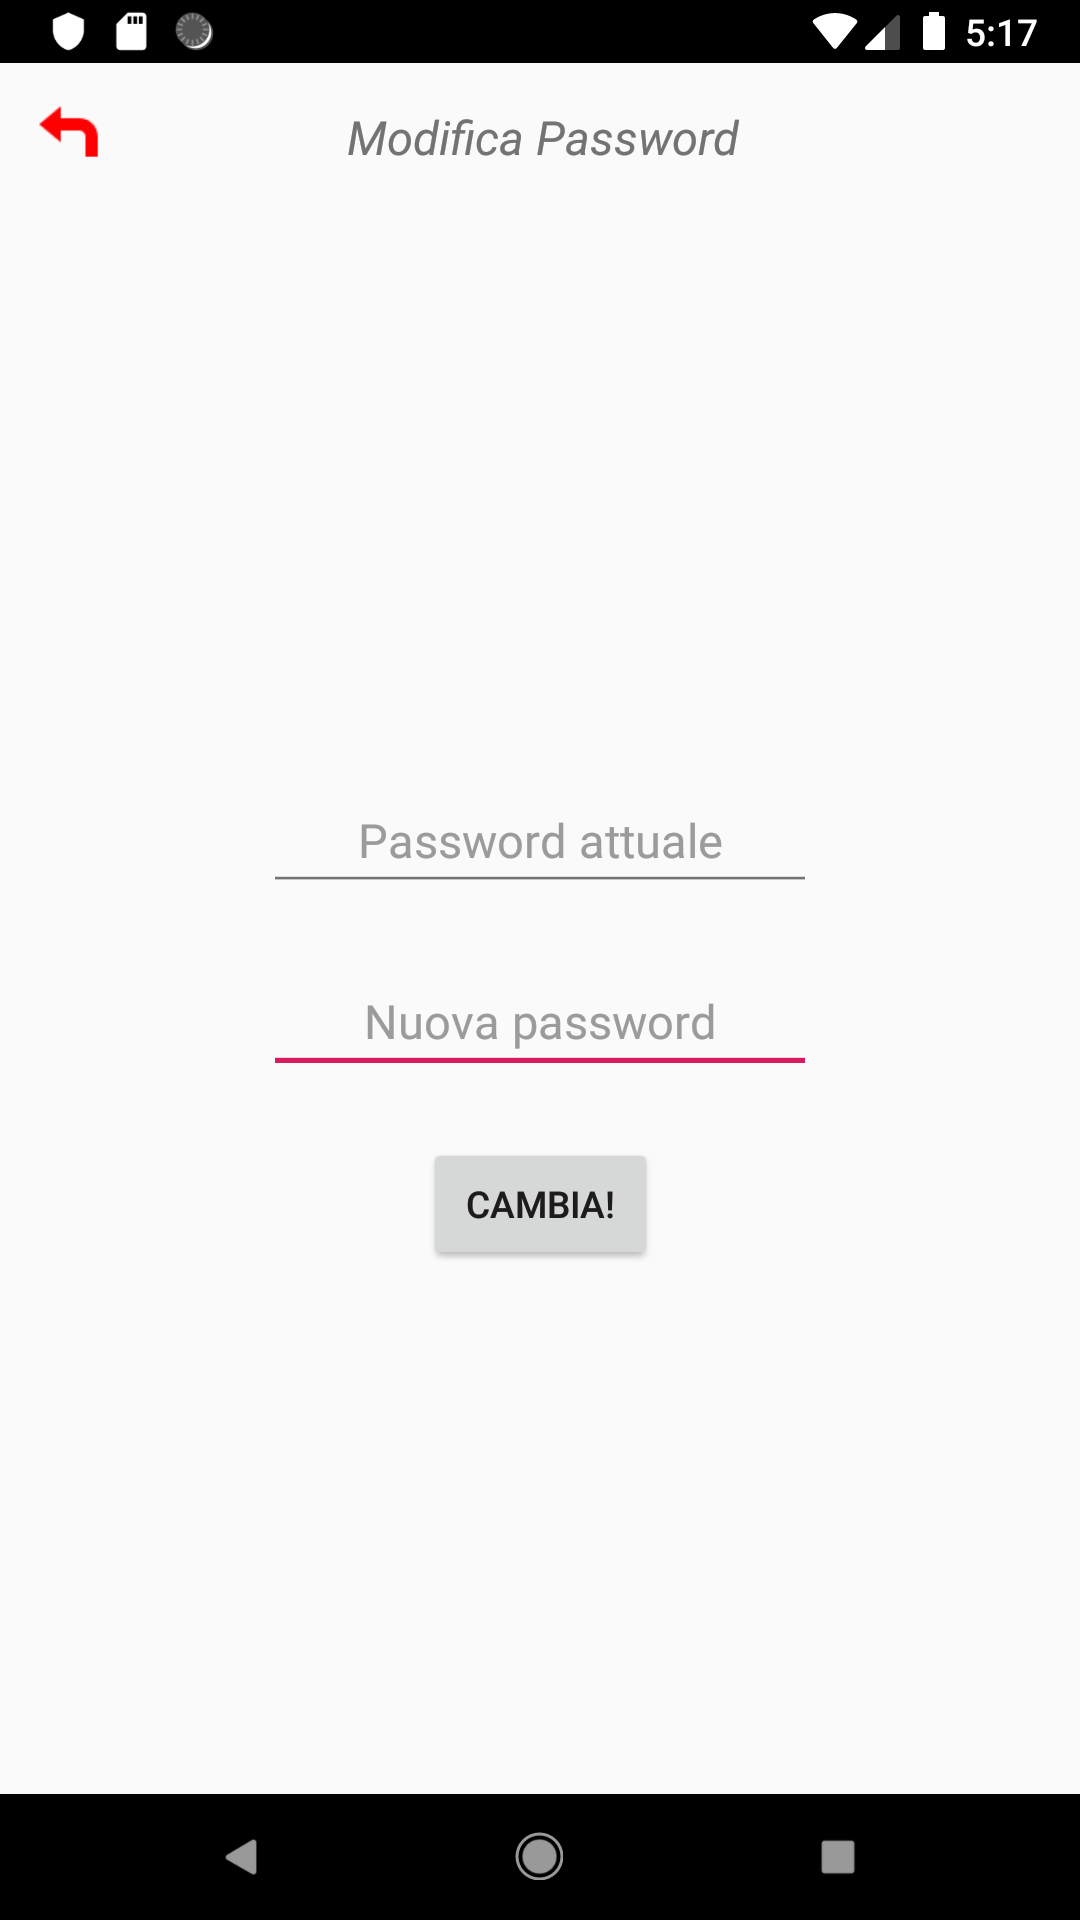
\includegraphics[width=.30\textwidth]{impostazioni_password}} \quad
	{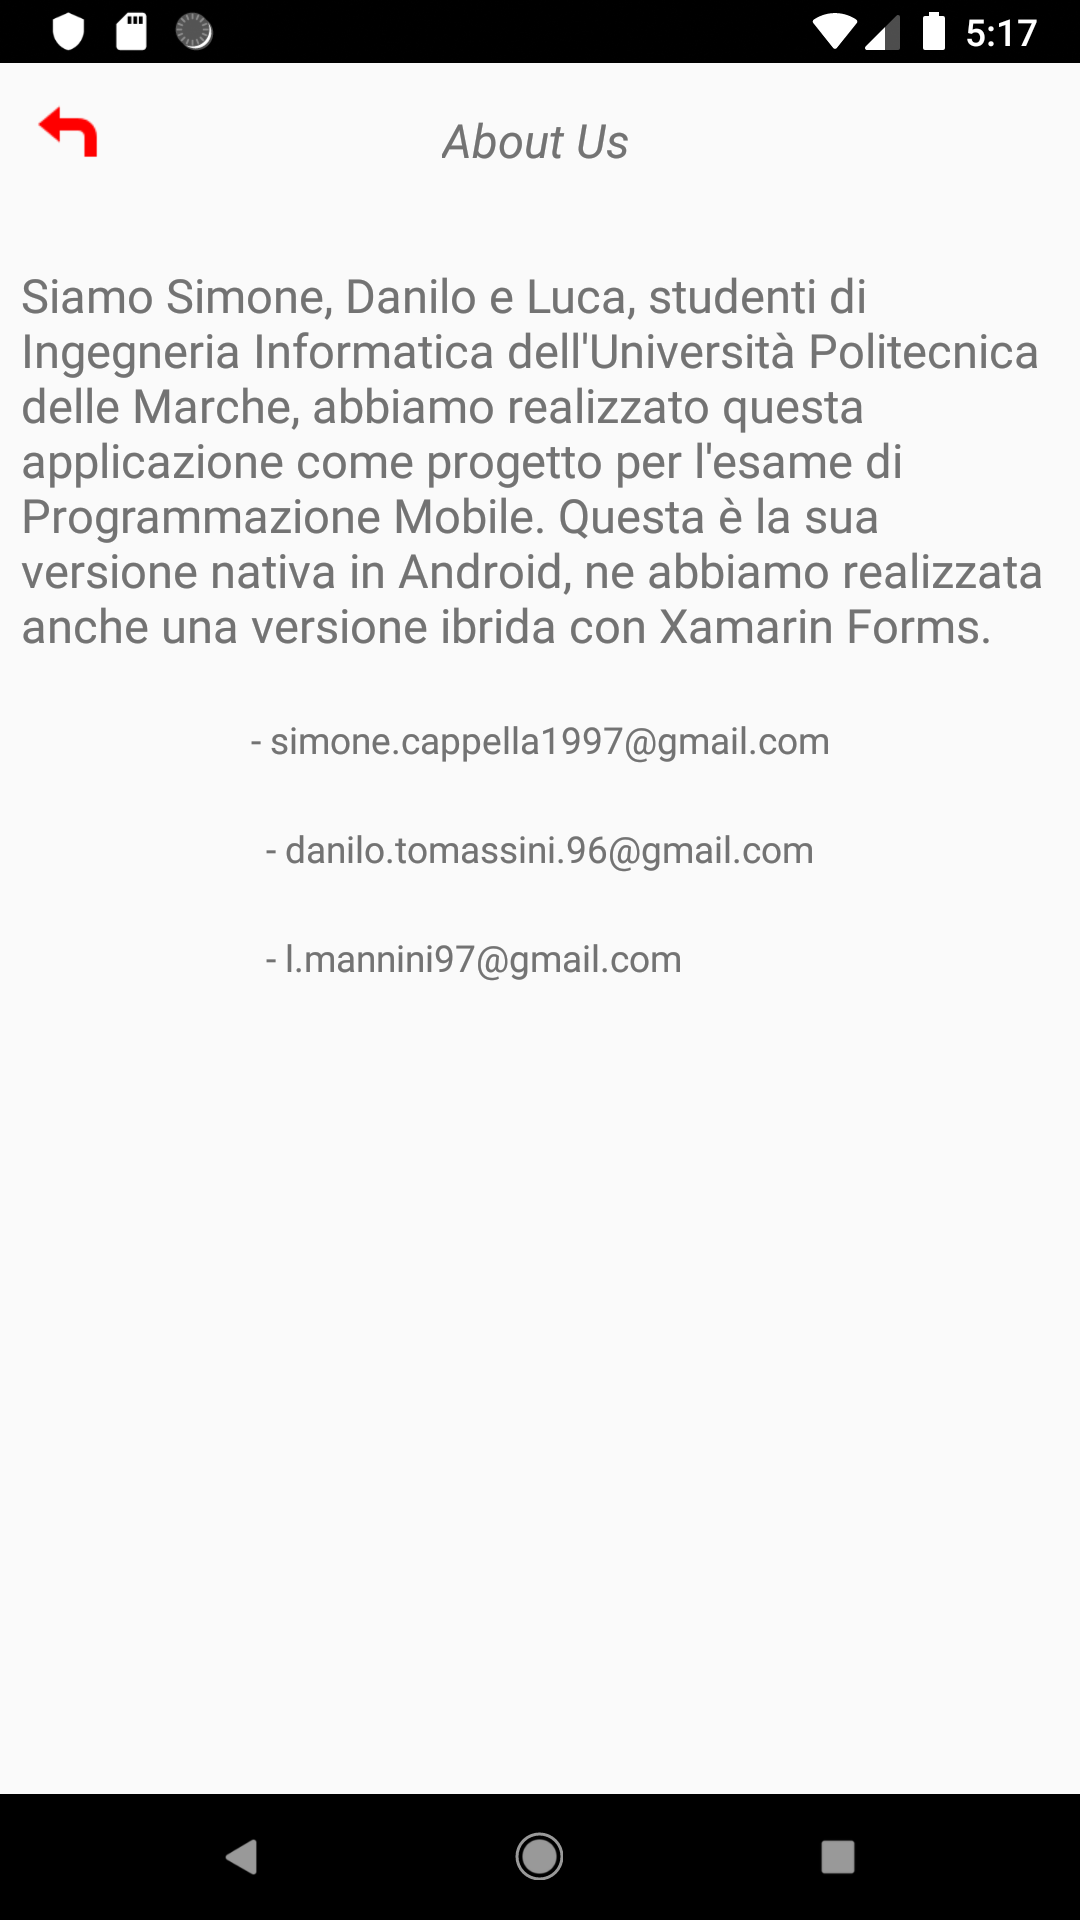
\includegraphics[width=.30\textwidth]{impostazioni_about_us}}
	\caption{\small Azioni eseguibili nelle impostazioni.}
\end{figure}
\newpage
\section{Implementazioni Android studio}
\subsection{Login e Registrazione}
Per avviare il login, ovviamente, è necessario riempire le \textbf{EditText} relative a username e password; i relativi valori verranno assegnati alle variabili \textbf{login\_name} e \textbf{login\_pass}.

La connessione al database viene instaurata indicando \textbf{method}, stringa inizializzata in precedenza a \textbf{"login"}, dati relativi ad username e password e l'url contenente il percorso fino alla funzione di login contenuta nel server.

Se la funzione del server da esito negativo non verrà effettuato il login e verrà stampato un \textbf{Toast}, per mezzo della funzione \textbf{show}. Altrimenti verrà stampato un messaggio di benvenuto e verrà lanciata la \textbf{MainActivity}.
\begin{lstlisting}
\\FirstActivity\\
[...]
public void userLogin(View view) {
[...]
try {
	Sring url = "http://mobileproject.altervista.org/login.php";
	auth = supportTask.execute(method, login_name, login_pass, url).get();
	} catch (ExecutionException e)
	{
		e.printStackTrace();
	}catch (InterruptedException a)
	{
		a.printStackTrace();
	}
	if(auth.equals("Login Success"))
	{
		launchMainActivity(view);
		show("Benvenuto "+ login_name + "!");
		finish();
	}else
	{
		show("Dati errati. Riprova.");
	}
}
[...]
\end{lstlisting}

La registrazione viene gestita in modo simile.

In un \textbf{if} viene verificato in modo veloce se le condizioni su username e password sono verificate, in caso contrario viene lanciato un avviso.

Il metodo con cui si instaura la connessione al server è lo stesso, cambiano solo gli argomenti, \textbf{url} e \textbf{method}.

Una volta che la registrazione è andata a buon fine l'attività viene interrotta e si torna alla schermata di login.

\begin{lstlisting}
\\Register\\
[...]
public void userRegister() {
[...]
if (register_name.length() >= 3 && register_pass.length() >= 3)
{
	try {
		String url = "http://mobileproject.altervista.org/register.php";
		auth= supportTask.execute(method, register_name, register_pass, url).get();
	} catch (ExecutionException e) {
		e.printStackTrace();
	} catch (InterruptedException e) {
		e.printStackTrace();
	}
	if (auth.equals("Registrazione avvenuta con successo!")) {
		show("Registrazione effettuata con successo, accedi!");
		finish();
	} else if (auth.equals("Username in uso")) {
		show("Username gia' in uso, prova con uno diverso!");
	}
}
else
{
show(I campi devono contenere almeno 3 caratteri.);
}
[...]
\end{lstlisting}

\subsection{Orario}
Avviata l'activity \textbf{orario} vengono catturate le dimensioni del display, calcolata la dimensione del \textbf{fragment} contenente la tabella dell'orario e fatto partire uno switch sul giorno corrente.

\begin{lstlisting}
\\Clock\\
[...]
protected void onCreate(Bundle savedInstanceState) {
[...]
Calendar calendar = Calendar.getInstance();
int day = calendar.get(Calendar.DAY_OF_WEEK);
Fragment fragment = null;
switch (day){
	case Calendar.MONDAY:
		fragment = new lun_fragment();
		nav.setSelectedItemId(R.id.lun);
		break;
	case Calendar.TUESDAY:
		fragment = new mar_fragment();
		nav.setSelectedItemId(R.id.mar);
		break;
	case Calendar.WEDNESDAY:
[...]
}
loadFragment(fragment);
[...]
\end{lstlisting}

Questo switch permette di caricare il fragment relativo al giorno corrente (es. se oggi è lunedì viene caricato il fragment relativo a lunedì); viene, infatti, inizializzato l'oggetto fragment e viene selezionato l'elemento sulla navbar.

\begin{lstlisting}
\\Clock\\
[...]
public boolean onNavigationItemSelected(@NonNull MenuItem item) {
Fragment fragment = null;
switch(item.getItemId())
{
	case R.id.lun:
		next = 0;
		fragment = new lun_fragment();
		break;
	case R.id.mar:
		next = 1;
		fragment = new mar_fragment();
		break;
	case R.id.mer:
		next = 2;
		fragment = new mer_fragment();
		break;
[...]
}
return loadFragment(fragment);
[...]
\end{lstlisting}

Allo stesso modo la funzione \textbf{onNavigationItemSelected}, associa in base allitem della navbar cliccato un'istanza del fragment all'oggetto fragment e nuovamente viene lanciata la funzione \textbf{loadFragment}.

La funzione \textbf{loadFragment} carica il fragment richiesto e gestisce lo scorrimento a destra o sinistra dipendentemente dalla posizione del fragment corrente rispetto a quello scelto.
\subsubsection{Fragment}
Prendiamo come riferimento il fragment relativo al \textbf{lunedì}, gli altri saranno implementati in modo analogo.

All'interno del fragment vengono nuovamente catturate le dimensioni del display e impostate le dimensioni delle varie caselle della tabella, rispettivamente:
\begin{itemize}
\item \textbf{Ora:} l'ora di inizio della lezione.
\item \textbf{Materia:} la materia inserita.
\item \textbf{Aula:} l'aula nel quale si terrà la lezione.
\item \textbf{X:} edit per cancellare la riga.
\end{itemize}

La tabella viene inizializzata nella funzione \textbf{onCreate}, qui, ogni elemento della tabella viene assegnato ad una variabile e successivamente "riempito" con il testo salvato, andadolo a recuperare con l'oggetto \textbf{sa}, della classe \textbf{SalvaOrario}, passando la chiave $\{lun\_1, lun\_2,..., lun\_11\}$ per quanto riguarda la tabella di lunedì, per la tabella di martedì le chiavi saranno costruite come $\{mar\_1,...,mar\_11\}$; la stessa logica vale per gli altri giorni; in tal modo possiamo recuperare in modo distinto le 11 materie salvate con la relativa aula per i diversi giorni.

\begin{lstlisting}
\\lun_fragment\\
[...]
public View onCreateView(LayoutInflater inflater, 
@Nullable ViewGroup container, @Nullable Bundle savedInstanceState) {
[...]
SalvaOrario sa = new SalvaOrario();
[...]
txtMat1 = v.findViewById(R.id.materia1);
txtMat1.setText(sa.getMateria("lun_1", getActivity()));
txtMat1.setOnClickListener(this);
txtAula1 = v.findViewById(R.id.aula1);
txtAula1.setText(sa.getAula("lun_1", getActivity()));
txtOra1 = v.findViewById(R.id.ora1);

txtMat2 = v.findViewById(R.id.materia2);
txtMat2.setText(sa.getMateria("lun_2", getActivity()));
txtMat2.setOnClickListener(this);
txtAula2 = v.findViewById(R.id.aula2);
txtAula2.setText(sa.getAula("lun_2", getActivity()));
txtOra2 = v.findViewById(R.id.ora2);
[...]
\end{lstlisting}

Nella funzione \textbf{onClick} viene gestita la scelta di inserire una materia nell'orario o eliminarne una dallo stesso. C'è, infatti, uno switch che gestisce il "click" nelle diverse sezioni della tabella. Abbiamo due diversi tipi di azione:
\begin{itemize}
\item \textbf{Aggiungere una materia:} per aggiungere una materia si seleziona un campo materia relativo all'ora in cui vogliamo inserirlo, questo attiverà l'elemento corrispondente nello switch che imposterà la variabile $n$, utilizzata successivamente per costruire la chiave e salvare nella classe SalvaOrario, la variabile $ora$, presa direttamente dalla view e chiama la funzione \textbf{launchList()}.
\item \textbf{Elimina una materia:} se viene selezionata la "X" sulla destra della tabella viene semplicemente "pulita" la riga corrispondente, infatti, nello switch, captato l'$edit$ corrispondente, viene impostata di nuovo la variabile $n$ per essere usata come chiave e le voci $materia$ e $aula$ vengono messe a $null$, viene lanciata, poi, la funzione \textbf{inserisciSalva()}; (la variabile $inc$ serve successivamente per inserire in un colpo solo più ore della stessa materia).
\end{itemize}
\newpage
\begin{lstlisting}
\\lun_fragment\\
[...]
public void onClick (View v) {
switch (v.getId())
{
	case R.id.materia1:
		n = 1;
		ora = txtOra1.getText().toString();
		v.startAnimation(buttonClick);
		launchList();
		break;
	case R.id.materia2:
		n = 2;
		ora = txtOra2.getText().toString();
		v.startAnimation(buttonClick);
		launchList();
		break;
[...]
	case R.id.edit1:
		n = 1;
		v.startAnimation(buttonClick);
		materia = null;
		aula = null;
		inc = 1;
		inserisciSalva();
		break;
	case R.id.edit2:
		n = 2;
		v.startAnimation(buttonClick);
		materia = null;
		aula = null;
		inc = 1;
		inserisciSalva();
		break;
[...]
\end{lstlisting}

La finzione \textbf{launchList}, chiamata nel momento in cui si vuole aggiungere una materia all'orario non fa altro che lanciare un \textbf{intent esplicito}, questo ci permette di scambiare dati tra l'activity chiamante e la chiamata, infatti tra i parametri della funzione \textbf{putExtra} abbiamo una chiave, $giorno\_ora$ e un valore, $"lunedi'" + ora$ ($ora$ è stata assegnata in precedenza nello switch). Inoltre c'è bisogno di un $REQUEST\_CODE$ utilizzato come chiave di riconoscimento tra le activity.

\begin{lstlisting}
\\lun_fragment\\
[...]
public static final int REQUEST_CODE = 0000;
[...]
public void launchList() {
	Intent intent = new Intent (getActivity(), List.class);
	intent.putExtra("giorno_ora", "lunedi'  " + ora);
	startActivityForResult(intent, REQUEST_CODE);
}
\end{lstlisting}

L'activity \textbf{List} genera la lsita predefinita delle materie da cui si può scegliere quella da inserire nella casella dell'orario scelta.

Qui i dati vengono recuperati proprio grazie alla chiave $giorno\_ora$, successivamente vengono istaziati $myDialog$ e $adapter$.

La funzione \textbf{setOnItemClickListener} chiamata per mezzo dell'oggetto $listMaterie$ e la successiva \textbf{OnItemClick} permettono di captare quale materia della lista viene scelta grazie alla sua posizione nella lista stessa.

Scelta la materia viene aperta la finestra di dialogo, all'interno di questa vengono definiti diversi elementi come una editText per l'aula e due bottoni, $- +$, questi permettono di incrementare e decrementare le ore di lezione relative alla materia.

Una volta inserita l'aula e il numero di ore si provede al salvataggio. Un listener sul bottone $btnSalva$ fa si che quando venga restituito il risultato all'activity chiamante con la variabile $intent$, questa contiene la materia scelta, l'aula e la conta delle ore, l'attivity termina con finish().
Una cosa analoga avviene nel momento in cui si decide tramite l'apposito bottone di inserire una nuova materia non contenuta nella lista predefinita.

\begin{lstlisting}
\\List\\
[...]
Intent intent = getIntent();
String giorno_ora = intent.getStringExtra("giorno_ora");
[...]
myDialog = new Dialog(this);
final ArrayAdapter<String>  adapter = new ArrayAdapter<>(this,
android.R.layout.simple_list_item_1, android.R.id.text1, listItem);
listMaterie.setAdapter(adapter);
[...]
listMaterie.setOnItemClickListener(new AdapterView.OnItemClickListener() {
	@Override
	public void onItemClick(AdapterView<?> parent, View view, int position,
	long id) {
		value = adapter.getItem(position);
[...]
myDialog.show();
[...]
btnMeno.setOnClickListener(new View.OnClickListener() {
	@Override
	public void onClick(View v) {
		i--;
		textContatore.setText(Integer.toString(i));
	}
}
[...]
btnPiu.setOnClickListener(new View.OnClickListener() {
	@Override
	public void onClick(View v) {
	i++;
	textContatore.setText(Integer.toString(i));
	}
}
[...]
btnSalva.setOnClickListener(new View.OnClickListener() {
	@Override
	public void onClick(View v) {
[...]
		Intent intent = new Intent();
		intent = intent.putExtra("mat", valore);
		setResult(Activity.RESULT_OK, intent);
		finish();
		myDialog.dismiss();
	}
[...]
\end{lstlisting}

La funzione \textbf{onActivityResult} si occupa di reperire dall'activity Lsit i risultati ottenuti dalla scelta. L'array di stringhe $res$ contiene ora nella posizione 0 la materia, nella posizione 1 l'aula e nella posizione 2 il numero di ore, che va "parsato" in un intero in quanto arrivava come una Stringa.

Viene considerato il caso in cui non si completa la scelta, in tal caso nell'activity Lista viene impostato il nome della materia a $back$ e non viene eseguita nessun'altra azione, la routine si interrompe. Nel caso in cui la scelta è stata completata i dati raccolti andranno salvati, sono passati, dunque, alla funzione \textbf{salvaOrario}.

\begin{lstlisting}
\\lun_fragment\\
[...]
public void onActivityResult(int requestCode, int resultCode, Intent data){
	super.onActivityResult(requestCode, resultCode, data);
	if ((requestCode == REQUEST_CODE) && (resultCode == Activity.RESULT_OK)) {
		String[] res = data.getStringArrayExtra("mat");
		materia = res[0];
		aula = res[1];
		inc = Integer.parseInt(res[2]);
	}
	if (materia.equals("back")){}
	else{
		salvaOrario(i, materia, aula);
	}
}
[...]
\end{lstlisting}

La funzione \textbf{salvaOrario} va a definire un cursore che sarà popolato con l'elemento del database trovato dal metodo \textbf{searchM} (questo trova nel database l'elemento il cui campo materia ha lo stesso nome della materia inserita).
Questo cursore permette di verificare, grazie all'$if$ se la materia inserita è gia presente nel database contenente le materie, in caso positivo il vecchio elemento viene eliminato; successivamente si inserisce nel database delle materie il nuovo elemento e viene chiamata la funzione \textbf{inserisciSalva()}.

Le materie vengono inserite nel database delle materie per permettere alla sezione $miei appunti$ di rendere disponibili le materie inserite nell'orario.

\begin{lstlisting}
\\lun_fragment\\
[...]
public void salvaOrario (String key, String materia, String aula) {
	Cursor c;
	c = dm.searchM(materia);
	if (c.getCount() > 0) {
		dm.delete(materia);
	}
	dm.insert(materia, ora, aula, key);
	inserisciSalva();
[...]
\end{lstlisting}

La funzione \textbf{inserisciSalva} permette di salvare, nuovamente tramite i metodi della classe \textbf{Salva Orario}, materia e aula scelti e nuovamente di aggiornare i valori delle $txtMat$ e $txtAula$.

Il \textbf{while} all'interno della funzione ripete il ciclo finchè la variabile $inc$ che conteneva la conta delle ore non arriva a 0; la Stringa $q$ viene costruita in modo da diventare una chiave per i metodi della classe SalvaOrario, infatti la variabile $i$ contiele la stringa "lun\_" e la variabile $n$ contiene il numero dipendentemente dalla riga scelta dalla tabella. Le variabili $n$ ed $inc$ alla fine del ciclo vengono rispettivamente incrementata e decrementata, questo permette di salvare in un solo colpo stessa materia e stessa aula all'interno della tabella, infatti il numero dell'elemento della tabella incrementa finche non si esaurisce il numero di ore deciso nella finestra di dialogo nell'activity List.

Lo \textbf{switch} su $n$ ha il compito di aggiornare immediatamente il valore della tabella nella posizione $n$.
\begin{lstlisting}
\\lun_fragment\\
[...]
public void inserisciSalva(){
	while (inc > 0){
		String q = i + n;
		sa.setMateria(q, materia, getActivity());
		sa.setAula(q, aula, getActivity());
		switch (n){
			case 1:
				txtMat1.setText(sa.getMateria(q, getActivity()));
				txtAula1.setText(sa.getAula(q, getActivity()));
				break;
			case 2:
				txtMat2.setText(sa.getMateria(q, getActivity()));
				txtAula2.setText(sa.getAula(q, getActivity()));
				break;
[...]
	}
	n++;
	inc--;
}
[...]
\end{lstlisting}

La classe \textbf{SalvaOrario} gestisce salvataggio ed estrazione per mezzo delle \textbf{SharedPreferences} di materia e aula.

Al suo interno sono presenti, infatti, quattro metodi:
\begin{itemize}
\item \textbf{setMateria:} prende tra gli argomenti chiave e materia e va a salvare la materia con tale chiave.
\item \textbf{getMateria:} va ad estrarre dai salvataggi la materia corrispondente alla chiave di ricerca.
\item \textbf{setAula:} di nuovo prende tra gli argomenti chiave ed aula (in questo caso la chiave viene combinata con la stringa $"\_A"$ per caratterizzare le chiavi relative alle aule) salva, dunque, il nome dell'aula.
\item \textbf{getAula:} estrae l'aula dai salvataggi per mezzo della chiave combinata con la stringa di cui sopra.
\end{itemize}

\begin{lstlisting}
\\SalvaOrario\\
[...]
public static void setMateria(String key, String value,  Context context) {
	SharedPreferences.Editor editor = preferences.edit();
	editor.putString(key, value);
	editor.commit();
}
public static String getMateria(String key, Context context)
{
	return preferences.getString(key, null);
}
public static void setAula(String key, String value,  Context context) {
	SharedPreferences.Editor editor = preferences.edit();
	editor.putString(key+"_A", value);
	editor.commit();
}
public static String getAula(String key, Context context) {
	return preferences.getString(key+ "_A", null);
}
\end{lstlisting}

\newpage
\subsection{I miei appunti}
\subsection{Appunti condivisi}
\subsection{Impostazioni}

\section{Implementazioni Xamarin}
\subsection{Login e Registrazione}
\subsection{Orario}
\subsection{I miei appunti}
\subsection{Appunti condivisi}
\subsection{Impostazioni}










































\end{document}